%% This is file `elsarticle-template-1-num.tex',
%%
%% Copyright 2009 Elsevier Ltd
%%
%% This file is part of the 'Elsarticle Bundle'.
%% ---------------------------------------------
%%
%% It may be distributed under the conditions of the LaTeX Project Public
%% License, either version 1.2 of this license or (at your option) any
%% later version.  The latest version of this license is in
%%    http://www.latex-project.org/lppl.txt
%% and version 1.2 or later is part of all distributions of LaTeX
%% version 1999/12/01 or later.
%%
%% The list of all files belonging to the 'Elsarticle Bundle' is
%% given in the file `manifest.txt'.
%%
%% Template article for Elsevier's document class `elsarticle'
%% with numbered style bibliographic references
%%
%% $Id: elsarticle-template-1-num.tex 149 2009-10-08 05:01:15Z rishi $
%% $URL: http://lenova.river-valley.com/svn/elsbst/trunk/elsarticle-template-1-num.tex $
%%
% \documentclass[preprint,12pt]{elsarticle}

%% Use the option review to obtain double line spacing
%% \documentclass[preprint,review,12pt]{elsarticle}

%% Use the options 1p,twocolumn; 3p; 3p,twocolumn; 5p; or 5p,twocolumn
%% for a journal layout:
%% \documentclass[final,1p,times]{elsarticle}
%% \documentclass[final,1p,times,twocolumn]{elsarticle}
%  \documentclass[final,3p,times]{elsarticle}
 \documentclass[final,3p,times,twocolumn]{elsarticle}
%% \documentclass[final,5p,times]{elsarticle}
%% \documentclass[final,5p,times,twocolumn]{elsarticle}

%% if you use PostScript figures in your article
%% use the graphics package for simple commands
%% \usepackage{graphics}
%% or use the graphicx package for more complicated commands
%% \usepackage{graphicx}
%% or use the epsfig package if you prefer to use the old commands
%% \usepackage{epsfig}

\usepackage[utf8]{inputenc} 
%% The amssymb package provides various useful mathematical symbols
\usepackage{amssymb}
\usepackage{hyperref}
\usepackage{graphicx}
\usepackage{subcaption}
\usepackage{lscape}
\usepackage{amsmath}
\usepackage{multirow}
% if you have landscape tables
\usepackage[figuresright]{rotating}
\usepackage{lineno}
\usepackage{algorithm} 
\usepackage{algpseudocode} 
\usepackage{comment}
\usepackage{lineno}

\usepackage{natbib}
\bibliographystyle{abbrvnat}
\setcitestyle{authoryear,open={(},close={)},citesep={;}} 

\usepackage{calc}
\setlength{\footskip}{\paperheight
  -(1in+\voffset+\topmargin+\headheight+\headsep+\textheight)
  -0.95in}

% for SVG figures
\usepackage{svg}

% For using LuaLaTeX or XeLaTeX compilers instead of pdflatex (memory limit)
\usepackage{fontspec} 
\setmainfont{Times New Roman}

\usepackage{titlesec}
\titleformat{\section}{\normalfont\bfseries}{\thesection}{1em}{}
\titleformat{\subsection}{\normalfont\itshape}{\thesubsection}{1em}{}

% Placeholder for numbers that come from runs still in progress. Fill from
%   python scripts/aggregate_results.py --latex      (tables)
%   python scripts/benchmark_efficiency.py           (latency)
% and delete this macro once no \tbd remains.
\newcommand{\tbd}{\textemdash}


\begin{document}

\begin{frontmatter}

% \title{Automated Identification of Invasive Aquatic Plants Using Deep Neural Networks on Controlled Image Datasets}
\title{Improving Out-of-Distribution Aquatic Plant Classification from Limited Controlled Training Data Using Confidence-Aware Re-Evaluation}

\author[label1]{Aaryan Panigrahi}
\author[label1]{Fengying Dang}


\address{Fengying Dang (fdang1@mtu.edu) is the corresponding author}
\address[label1]{Department of Electrical and Computer Engineering, Michigan Technological University, Houghton, MI 49931, USA}


\begin{abstract}
 % Focus on why the problem is hard - limited data and complex env - current limitations
Aquatic invasive species (AIS) threaten the resilience of fisheries and aquaculture systems, causing severe ecological damage and economic losses. Accurate early identification is necessary to manage these species, and the long-term goal of this work is a classifier that runs on a camera-equipped underwater rover. Collecting high-quality images in underwater environments is difficult and expensive, so training sets are small and usually captured in the laboratory, and computer vision models trained on them often fail to generalize to the visual variations found in natural settings. This study addresses that gap with three ingredients. A compact ConvNeXt-V2 Tiny backbone (28~M parameters, 4.5~G multiply--adds per image) is kept frozen and only a parameter-efficient Gated Attention head (0.26~M weights) is trained, which suits the compute budget of an onboard computer. The `You Need To Look Twice' (YNLT) module, inspired by the human behavior of closely re-examining uncertain details, re-evaluates an image with multi-scale patches only when confidence, margin and entropy indicate an unreliable first look. Finally, the 203 laboratory photographs are complemented with 1{,}140 openly licensed field photographs of the same 21 Michigan species, drawn from GBIF-mediated iNaturalist observations and split by observation so that no plant appears in both training and test data. On a single laboratory split the gated head with YNLT raised accuracy from 84.78\% to 93.48\% in the laboratory and from 47.06\% to 64.71\% on 17 crowd-sourced field images. The combined protocol reports mean and standard deviation over five seeds on a laboratory test, a 210-image web test, and 42 held-out outdoor photographs, together with a learning curve that relates accuracy to the number of training images per class. These results indicate how laboratory and web imagery can be combined to identify invasive plants in complex environments with a model small enough for field deployment.
\end{abstract}

\begin{keyword}
Aquatic invasive species \sep Computer vision \sep precision agriculture \sep Domain generalization \sep Environmental monitoring
\end{keyword}

\end{frontmatter}

%%%%%%%%%%%%%%%%%%%%%%%%%%%%%%%%%%%%%%%%%%%%%%%%%%%%%%%%%%%%%%%%%%%%%%%%%%%%%%%%%%%%%%%%%%%%%%%%%%%%%%%%%%%%%%%%%%%%%%%%%%%%%%%%%%%%%%
%% main text
\section{Introduction}
\label{sec:intro}

Invasive species threaten biosecurity, agriculture, and human health, with global control and damage costs estimated in the trillions of dollars~\cite{tasker2024nuanced, macedo2024economic, shen2024typical, vaissiere2022nature, cuthbert2021global}. In the United States, recent estimates place annual losses near \$138 billion, a large fraction of which is attributable to freshwater plants, especially submerged and floating taxa~\cite{pimentel2000environmental, lovell2006economic, warziniack2021economics, macedo2024economic}. In fisheries and aquaculture, dense mats of invasive macrophytes reduce dissolved oxygen, obstruct spawning habitat, clog equipment, and raise operating costs. Early, accurate identification is therefore a practical management need rather than a purely taxonomic one.

Existing identification methods do not scale to routine monitoring. Field identification depends on botanical expertise~\cite{dehez2023investigation}. Molecular assays are accurate but require specialized sampling and laboratory capacity~\cite{angles2019detection, ghahramanzadeh2013efficient, scriver2015development}. Remote sensing covers large areas but lacks the spatial detail needed to separate morphologically similar submerged species~\cite{brooks2019implementing, unitis2018remote, jochems4883509active}. Image-based computer vision is attractive because it uses ordinary cameras~\cite{wang2026realtime}. The difficulty is not the camera; it is the data. High-quality underwater photographs are expensive to collect, so training sets are small and usually captured in the laboratory, while deployment images come from the field.

Prior aquatic plant classifiers show that convolutional networks can work when data are plentiful and classes are visually distinct, as in seagrass benchmarks~\cite{DeepSeaGrass1, Nawaz2025Seagrass, Paul2023LWDS, baos_cnn}. Freshwater monitoring in the Great Lakes is a different problem: native and invasive species often share the same coarse appearance, and only a few dozen labeled laboratory images may be available per study. Transfer learning from ImageNet, and earlier hierarchical SVMs for kelp~\cite{Kelps_SVMs}, reduce the data requirement but still collapse high-resolution botanical detail when images are resized to a standard $224\times 224$ input. The resulting models can look confident on laboratory photos and fail on handheld or in situ images of the same species.

Several computer-vision lines of work already try to ``look closer,'' but they are a poor fit for this regime. Recurrent attention models select a sequence of glimpses with reinforcement learning~\cite{mnih2014recurrent}. Coarse-to-fine and recurrent attention CNNs learn where to zoom for fine-grained recognition~\cite{fu2017look}. Multi-resolution networks and multi-crop test-time augmentation evaluate extra scales or crops for every image~\cite{krizhevsky2012imagenet, huang2018multiscale}. Attention-based fine-grained heads localize discriminative parts, typically on large bird or car datasets~\cite{fu2017look}. Hard-example mining reweights difficult samples during training~\cite{shrivastava2016training}. Uncertainty-aware and selective prediction methods either study calibration~\cite{Guoetal2017, Ovadiaetal2019, hendrycks2017baseline} or abstain when the model is unsure~\cite{geifman2017selective}. Learned zoom, always-on multi-crop, and abstention each assume either abundant labeled data, a budget to process every image at many scales, or the option to refuse a decision. None of those assumptions holds for laboratory-to-field aquatic identification, where missing an invasive plant is costly and the training set contains on the order of a hundred images.

The intended platform shapes the design. The classifier is meant to run on a camera-equipped underwater rover that surveys lake beds for invasive macrophytes, where the onboard computer has a fraction of the compute of a workstation GPU and must also run navigation and perception. This rules out large vision transformers and always-on multi-scale inference, and it argues for a compact convolutional backbone that is run once per image and only re-run where needed. We therefore build on ConvNeXt-V2 Tiny~\cite{Wooetal2023}: 28~M parameters and 4.5~G multiply--adds for a $224\times 224$ input, about a quarter of the cost of ViT-B/16 at the same input size (Table~\ref{tab:cost}), with smaller Nano, Pico and Atto members of the same family available if the final budget is tighter. The backbone is kept frozen, so only a head of 16~k to 262~k weights is trained, which both limits overfitting on a few hundred images and makes retraining for new species cheap.

This paper addresses that gap. We train only a small classification head on the frozen ConvNeXt-V2 backbone using laboratory images of 21 Michigan aquatic species, five of them invasive, and we evaluate on crowd-sourced field photographs that were never used for training. The proposed `You Need to Look Twice' (YNLT) module is a confidence-aware second look: if the first downsampled pass is ambiguous, the system extracts multi-scale patches and aggregates a weighted vote. A parameter-efficient gated attention head is used to suppress laboratory background features that do not transfer to the field. Errors are treated asymmetrically: failing to flag an invasive species (false negative) is treated as more serious than the reverse. Because the laboratory set alone provides only about six training images per species, we additionally assemble 1{,}140 openly licensed field photographs of the same species from GBIF-mediated iNaturalist observations and measure what training on laboratory images, web images, or both does to laboratory, web and outdoor test accuracy.

Our contributions are:
\begin{enumerate}
\item A small-data aquatic classification setting that explicitly measures controlled-to-field domain shift, rather than reporting only laboratory accuracy.
\item YNLT, a test-time module that spends extra computation only when confidence, margin, and entropy indicate an unreliable first look, instead of always cropping or abstaining.
\item A gated attention classification head, trained with a frozen backbone, that improves out-of-distribution accuracy relative to a linear classifier on the same features.
\item A web-sourced field image set for the same 21 species, with observation-grouped splits, and a data-source ablation (laboratory, web, both) with a learning curve that relates accuracy to the number of training images, answering how many samples the trained head needs.
\end{enumerate}

The remainder of the paper is organized as follows. Materials and methods are presented in Section~\ref{sec:materials_methods}. Results are reported in Section~\ref{sec:results}. Limitations and computational cost are discussed before the conclusions in Section~\ref{sec:conclu}.


\section{Materials and Methods}
\label{sec:materials_methods}

\subsection{Study area}
\label{subsec:study_area}

The geographic focus of this study is the state of Michigan, which encompasses portions of four Great Lakes (Lake Superior, Lake Michigan, Lake Huron, and Lake Erie) alongside numerous smaller inland lakes. These freshwater systems support highly diverse ecological communities, including a wide variety of native aquatic plant and fish species. However, the balance of these habitats is increasingly threatened by the introduction and proliferation of aquatic invasive plants. This study focuses on identifying 21 specific aquatic plant species found within this region, five of which are classified as invasive. Figure \ref{fig:map} illustrates the study area and the approximate occurrence distribution of these species.

\begin{figure*}[!h]
\centering
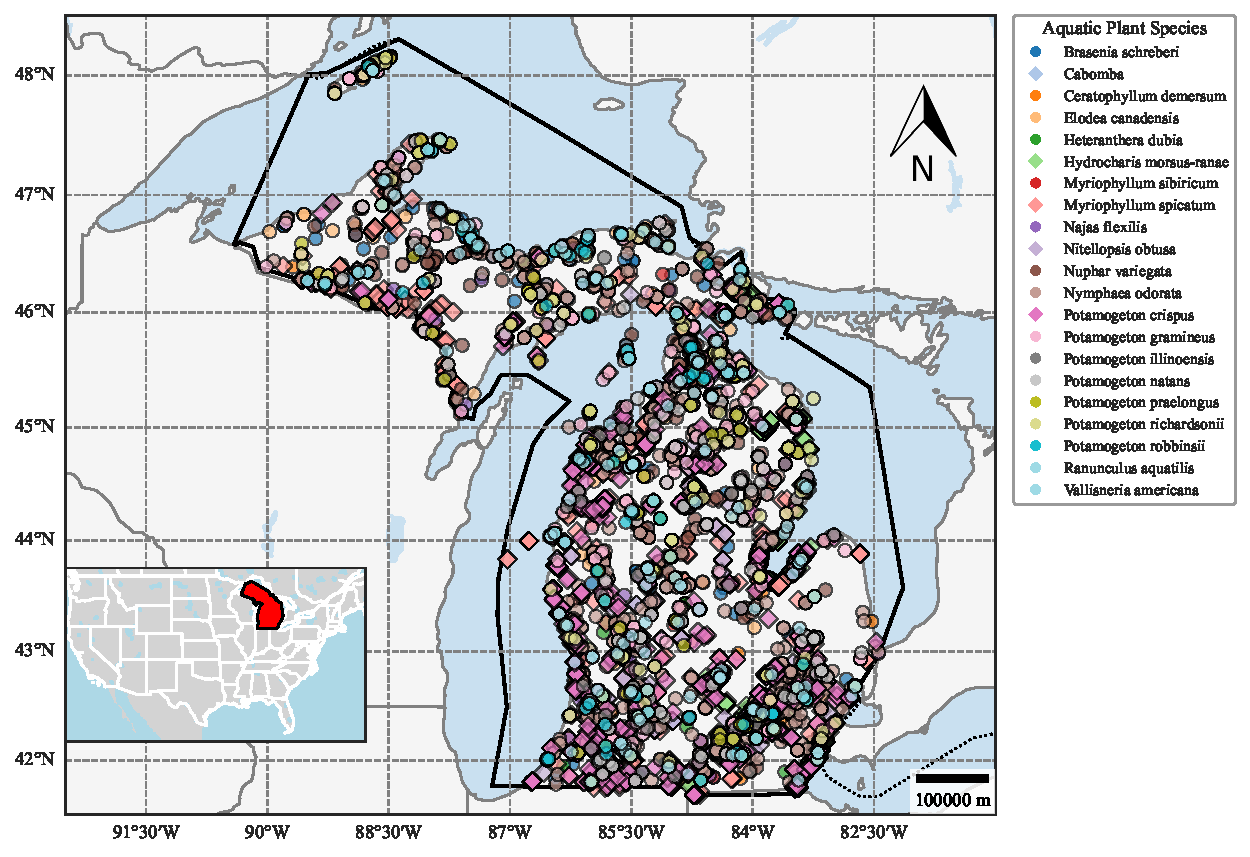
\includegraphics[width=1.0\textwidth]{figs/map.pdf}
\caption{Map of Michigan illustrating the geographic focus of the study. The approximate occurrences of 21 aquatic plant species are plotted based on data from the Global Biodiversity Information Facility (GBIF). The five invasive species are denoted by diamond markers, while the 16 native species are denoted by circular markers. The inset map (bottom left) indicates Michigan's location within the contiguous United States.} 
\label{fig:map}
\end{figure*}

\subsection{Dataset details}
Data collection in underwater environments is a recognized challenge. This study therefore uses three image collections of the same 21 species (Table~\ref{tab:data}): photographs captured in a controlled laboratory setting, openly licensed field photographs gathered from biodiversity databases, and a small set of outdoor photographs that is used only for testing.

\subsubsection{Laboratory images}
% \begin{figure*}[!ht]
% \centering
% 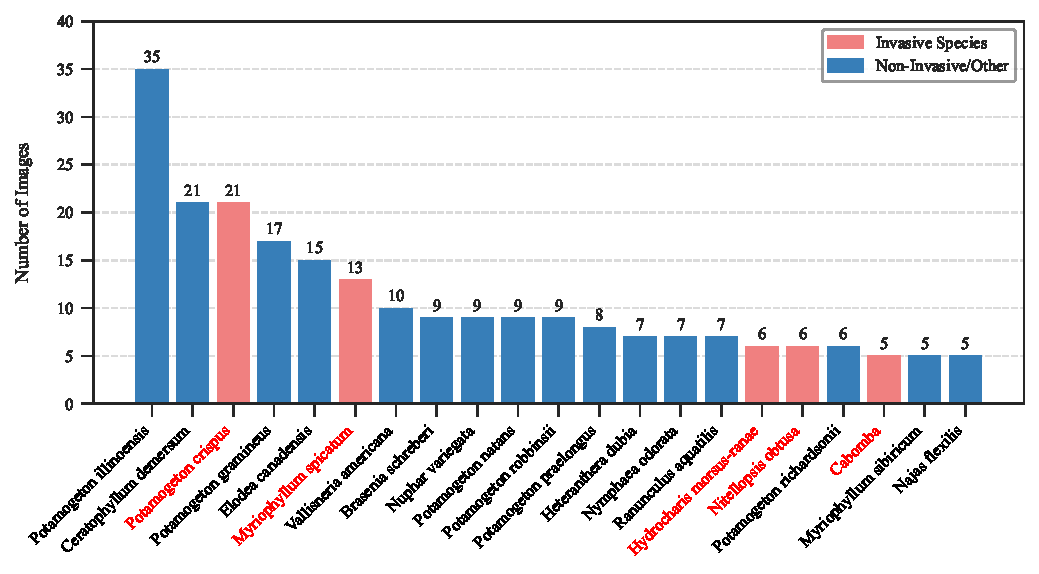
\includegraphics[width=1.0\textwidth]{figs/data_dist.pdf}
% \caption{Distribution of laboratory images across the 21 species.}
% \label{fig:data_dist}
% \end{figure*}

The laboratory collection behind the original experiment (Table~\ref{tab:ablation}) comprised 230 images across 21 plant species, 5 of which are invasive, split 60/20/20 by stratified sampling into 138 training and 46 validation and 46 test images. The copy available for the experiments in Sections~\ref{subsec:datagrid}--\ref{subsec:backbones} holds 203 of these photographs at $1500\times 1000$ pixels; several species have only two or three photographs, so a 60/20/20 stratified split leaves one training image for the rarest classes. Basic preprocessing removed reference artifacts such as coins and scales.

\subsubsection{Web-sourced field images}
\label{subsec:webdata}

Laboratory photographs alone give roughly six training images per species. To raise that number and to expose the classifier to field conditions during training, we queried the Global Biodiversity Information Facility (GBIF) for research-grade iNaturalist observations of each of the 21 species and downloaded the associated photographs. After removing duplicate photographs, the collection contains 1{,}140 images from 532 observations (32--106 images per species), 486 of them from the United States and 166 from Canada, with 38 from Michigan; the remainder come mainly from the Netherlands, Germany and Australia. Every image is stored with its licence and rights holder: 763 are CC~BY-NC, 124 CC~BY-NC-ND, 110 CC~BY, 77 CC0, and the rest CC~BY-ND, CC~BY-NC-SA or all-rights-reserved records that are used for research only and not redistributed. Image sizes range from $354\times 265$ to $2048\times 2048$ pixels, with a median width of 1{,}536.

An iNaturalist observation often carries several photographs of the same plant (up to 15 here; 861 of the 1{,}140 images belong to multi-photograph observations). Splitting by image would place photographs of one plant in both training and test sets. All splits are therefore made at the observation level, stratified per species, with 60\% of the images of each species for training and 20\% each for validation and test. The same procedure, seeded per species, is applied to the laboratory images, so the laboratory test images are identical whichever collection a model is trained on. Split lists are stored as CSV files with the released code.

\subsubsection{Outdoor test images}
The 42 outdoor photographs of hand-held plants (9 species, 16 of them \emph{Nuphar variegata}) are never used for training or model selection in the new protocol. They are the held-out field test. In the original experiment of Table~\ref{tab:ablation} a 33-image version of this set was divided equally between validation and test and used for checkpoint selection.

\begin{table}[!ht]
    \centering
    \caption{Images per species in the three collections. Invasive species are marked with an asterisk. Web images are counted after duplicate removal; the number of distinct iNaturalist observations is given in parentheses.}
    \label{tab:data}
    \renewcommand{\arraystretch}{1.1}
    \small
    \begin{tabular}{lrrr}
        \hline
        \textbf{Species} & \textbf{Lab} & \textbf{Web (obs.)} & \textbf{Outdoor} \\
        \hline
        Brasenia schreberi & 8 & 60 (25) & 0 \\
        Cabomba$^{*}$ & 5 & 53 (25) & 0 \\
        Ceratophyllum demersum & 21 & 52 (25) & 1 \\
        Elodea canadensis & 15 & 39 (26) & 0 \\
        Heteranthera dubia & 7 & 32 (25) & 0 \\
        Hydrocharis morsus-ranae$^{*}$ & 2 & 36 (26) & 0 \\
        Myriophyllum sibiricum & 4 & 70 (25) & 0 \\
        Myriophyllum spicatum$^{*}$ & 13 & 48 (26) & 3 \\
        Najas flexilis & 5 & 48 (25) & 0 \\
        Nitellopsis obtusa$^{*}$ & 5 & 54 (25) & 2 \\
        Nuphar variegata & 3 & 34 (25) & 16 \\
        Nymphaea odorata & 2 & 36 (26) & 1 \\
        Potamogeton crispus$^{*}$ & 20 & 67 (26) & 1 \\
        Potamogeton gramineus & 17 & 106 (25) & 7 \\
        Potamogeton illinoensis & 36 & 56 (25) & 0 \\
        Potamogeton natans & 8 & 38 (26) & 0 \\
        Potamogeton praelongus & 3 & 87 (25) & 0 \\
        Potamogeton richardsonii & 6 & 63 (25) & 6 \\
        Potamogeton robbinsii & 8 & 43 (25) & 0 \\
        Ranunculus aquatilis & 5 & 66 (26) & 5 \\
        Vallisneria americana & 10 & 52 (25) & 0 \\
        \hline
        Total & 203 & 1{,}140 (532) & 42 \\
        \hline
    \end{tabular}
\end{table}

\subsubsection{Preprocessing and Augmentation}

\begin{figure*}[!h]
\centering
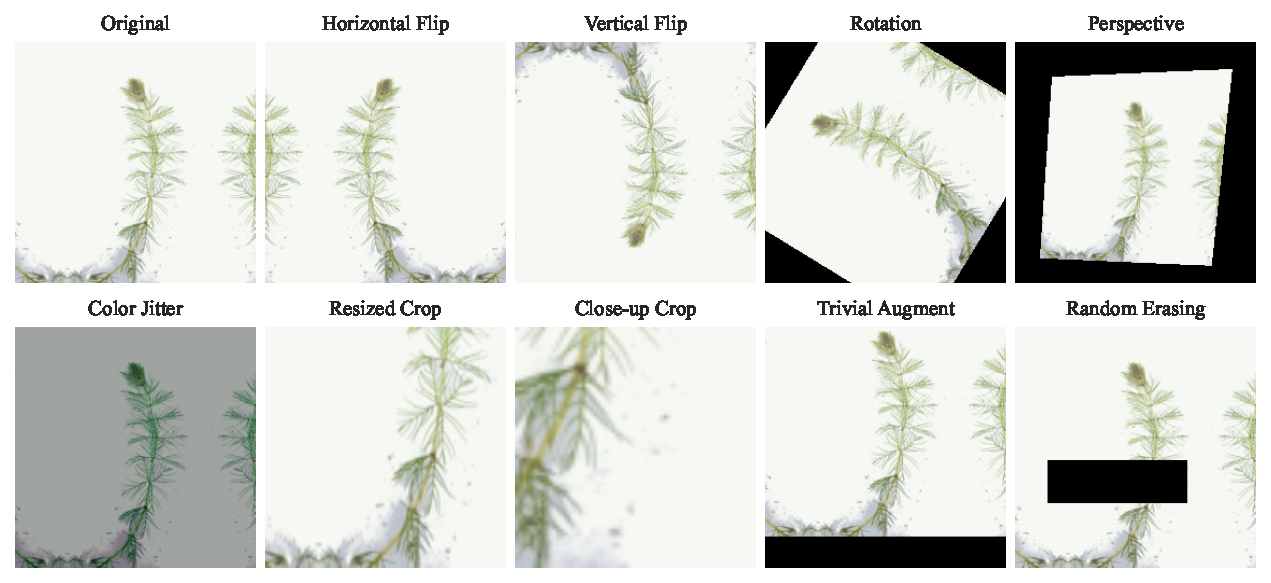
\includegraphics[width=0.9\textwidth]{figs/augmentations.pdf}
\caption{Various data augmentation techniques applied to the original images. The first row demonstrates basic geometric augmentations. The augmentations in the second row were specifically tuned to improve generalization from a small dataset. The close-up crop allows the model to learn from high-resolution details that would otherwise be lost during downsampling.} 
\label{fig:augmentations}
\end{figure*}

Given training sets of a few hundred images, a comprehensive data augmentation pipeline, illustrated in Figure \ref{fig:augmentations}, was critical. The same pipeline is applied to laboratory and web images.

The laboratory images were captured at high resolution (3000x4000 pixels originally, 1500x1000 in the copies used for retraining), whereas standard pretrained convolutional backbones are optimized for smaller input dimensions (e.g., 224x224 pixels) to limit parameter count and prevent overfitting. Downsampling the original images directly to these dimensions would result in the loss of fine botanical details. To preserve these details and fully utilize the high-resolution data, the model was trained on randomly cropped patches extracted from the original images. These patches, ranging from 20\% to 100\% of the original image area, were subsequently resized to 224x224 pixels. This approach preserves high-resolution features and induces scale invariance, preparing the model for downstream resolution-dependent modules.

Following the random crop, a series of geometric transformations, including rotations, flips, and affine transformations, were applied to simulate varied camera perspectives. Natural color, brightness, and lighting variations were also introduced. These transformations were applied with a probability of 0.5 using the Torchvision library. For the retraining experiments of Sections~\ref{subsec:datagrid}--\ref{subsec:curve} the same augmentation schedule (random resized crop with 10--100\% area, flips, rotation up to \(90^\circ\), perspective, colour jitter, TrivialAugment, random erasing) was re-implemented as batched GPU operations acting on images decoded once and stored at \(320\times 320\) pixels, so that the data pipeline, rather than the frozen encoder, no longer limited throughput; a 250-epoch run on 834 images takes about five minutes on the RTX 3070 Ti. The evaluation transform is a plain resize to \(224\times 224\) in both implementations.

The final augmentation stage involved random erasing, which masks a random rectangular region of the image. This technique prevents the model from relying on specific localized features, thereby encouraging the learning of more robust and generalized plant characteristics. Finally, the augmented images were normalized and converted to tensors prior to model training.

% \subsection{Plant Species Classification Method}

% \begin{figure}[!h]
% \centering
% 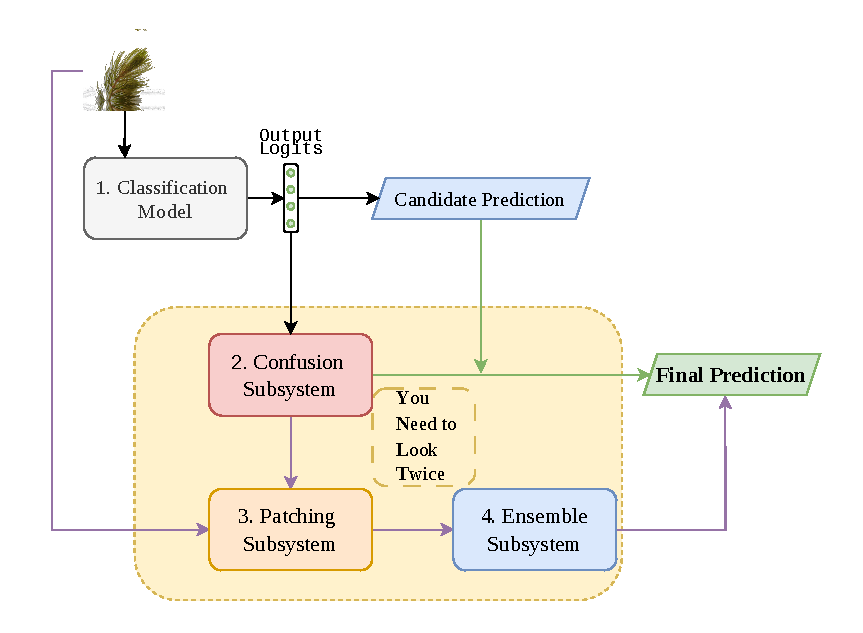
\includegraphics[width=0.5\textwidth]{figs/figs26/SimpleBlocksUpdated.drawio.pdf}
% \caption{Block diagram of the proposed Plant Species Classification Model. The image is first passed to the classification model, which outputs logits corresponding to each plant species. Based on this output, a candidate prediction as well as a corresponding evaluation of how confused the model is, is carried out. If the model is not confused, then the candidate prediction is finalized. Otherwise the Patching subsystem creates patches and passes them onto the ensemble subsystem, which makes the final prediction after a closer look.} 
% \label{fig:model_block}
% \end{figure}

% % \begin{figure*}[!h]
% % \centering
% % 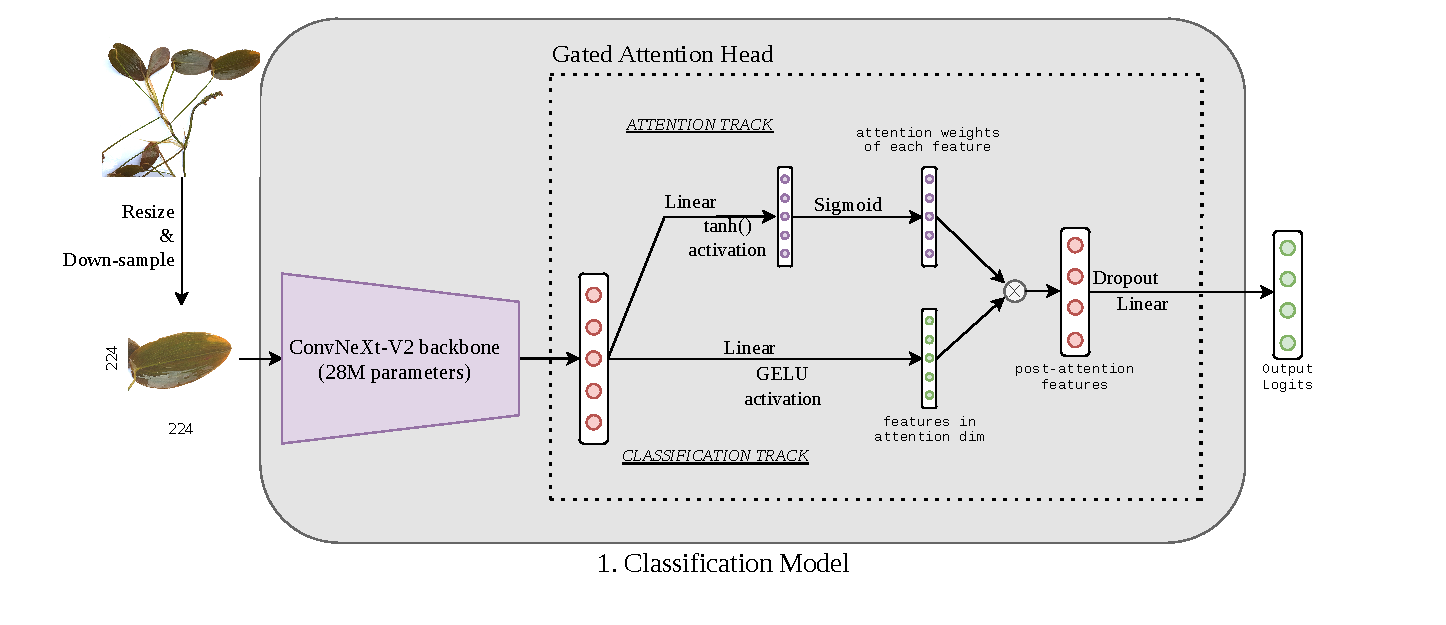
\includegraphics[width=1.0\textwidth]{figs/figs26/PlantClassification26.drawio.pdf}
% % \caption{The first stage in our proposed solution is a classification model. The input image is resized and fed to a pretrained ConvNeXt-v2 backbone for feature extraction. The output of the pretrained model is passed on to a our Gated-Attention classification head. This module has 2 parallel tracks - one for the classification features and another to compute the attention weights of those features. The outputs of both of these tracks are multiplied and the last layer outputs logits corresponding to each plant species.} 
% % \label{fig:model_block}
% % \end{figure*}


% % \begin{figure*}[!h]
% % \centering
% % 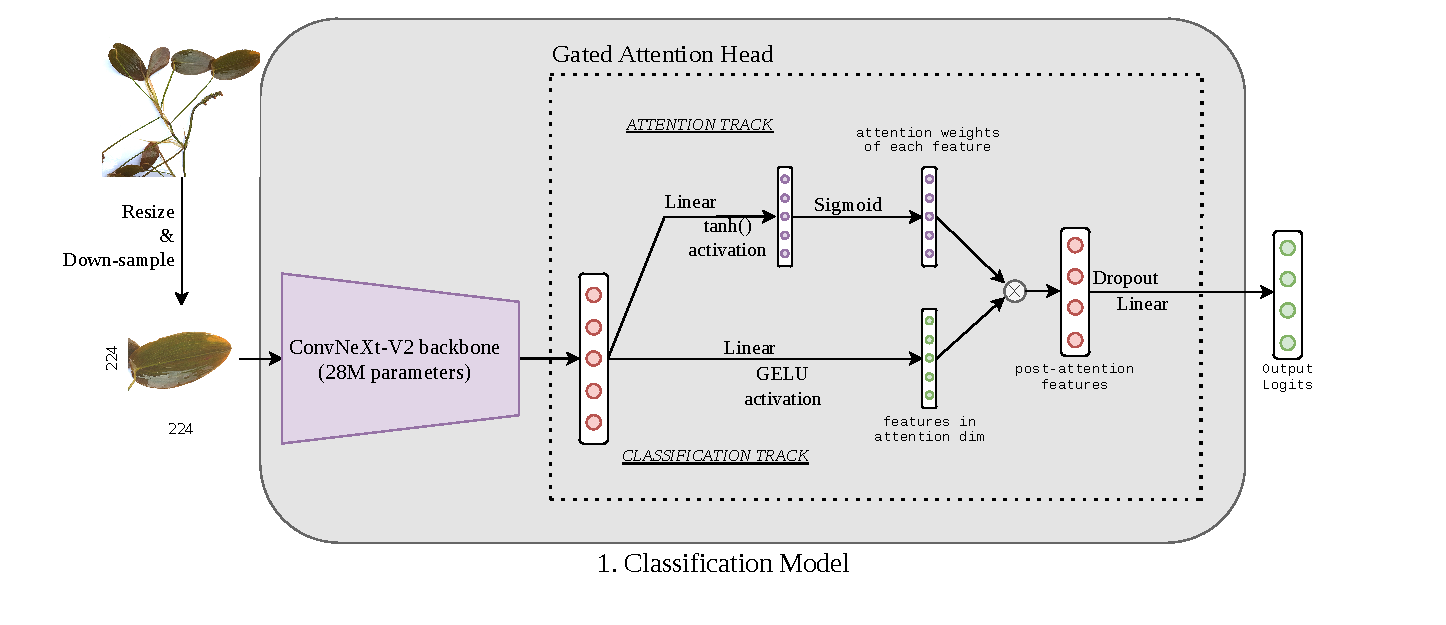
\includegraphics[width=1.0\textwidth]{figs/figs26/PlantClassification26.drawio.pdf}
% % \caption{The first stage in our proposed solution is a classification model. The input image is resized and fed to a pretrained ConvNeXt-v2 backbone for feature extraction. The output of the pretrained model is passed on to a our Gated-Attention classification head. This module has 2 parallel tracks - one for the classification features and another to compute the attention weights of those features. The outputs of both of these tracks are multiplied and the last layer outputs logits corresponding to each plant species.} 
% % \label{fig:model_block}
% % \end{figure*}


% \begin{figure*}[!h]
% \centering
% 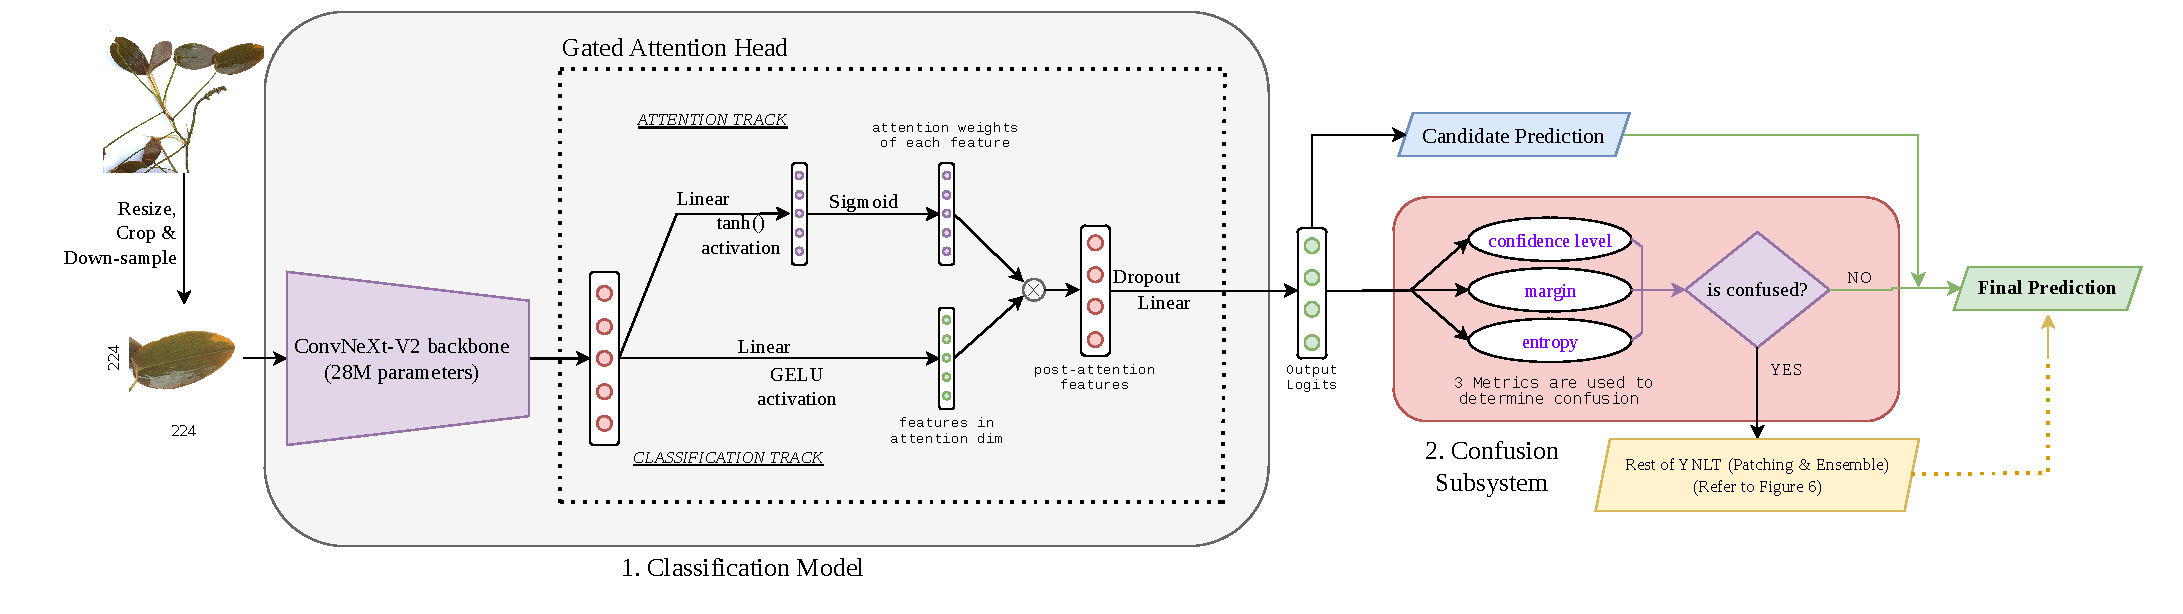
\includegraphics[width=1.0\textwidth]{figs/figs26/CombinedClassificatioAndConfusion.drawio.pdf}
% \caption{First 2 Modules} 
% \label{fig:model_block}
% \end{figure*}

\subsection{Plant Species Classification Method}

\begin{figure*}[!h]
\centering
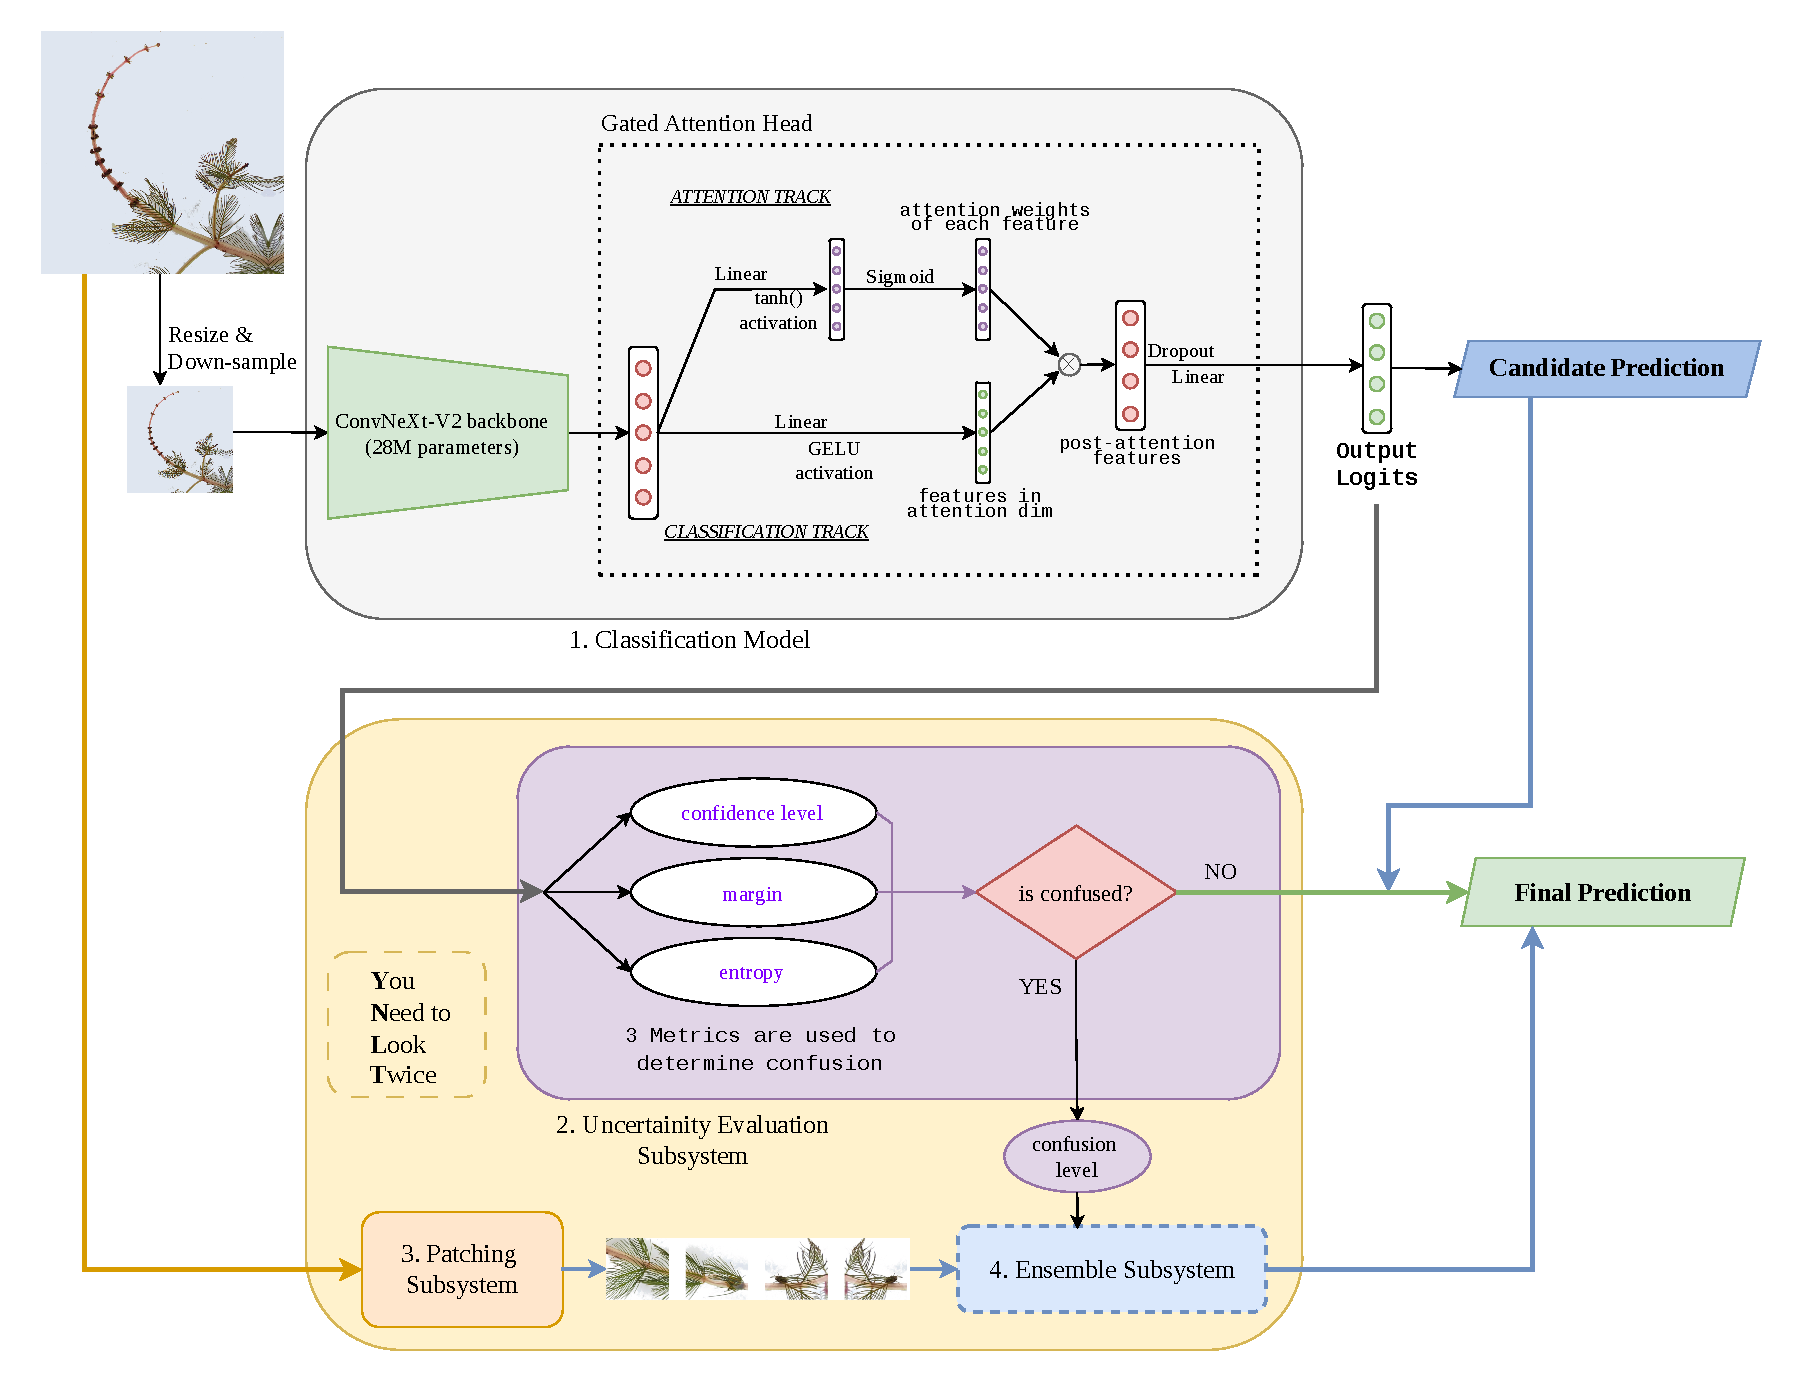
\includegraphics[width=1.0\textwidth]{figs/figs26/CombinedClassificatioAndConfusion_simplified.drawio.pdf}
\caption{Block diagram of the proposed Plant Species Classification pipeline. The system consists of two primary modules: (1) a feature extraction and classification network that outputs initial class logits, and (2) an uncertainty evaluation and ensembling system (YNLT) that assesses prediction confidence and re-evaluates the image using high-resolution patches if necessary.} 
\label{fig:model_block}
\end{figure*}

As illustrated in Figure \ref{fig:model_block}, the proposed architecture consists of two primary pathways. The first is the classification module, which processes an input image or patch to generate class-specific logits. The second module is the uncertainty evaluation system, which assesses the confidence of the initial prediction and, if necessary, triggers a high-resolution re-examination to finalize the classification.

\subsubsection{Pretrained ConvNeXt-V2 Backbone}

ConvNeXt-V2 integrates modern architectural advancements inspired by transformer models into a convolutional framework \cite{Wooetal2023}. It incorporates mechanisms such as larger convolutional kernels and global response normalization (GRN) while retaining the spatial inductive biases characteristic of standard convolutional operations. This architecture provides high representational capacity without introducing the excessive parameter count typically associated with pure transformer models. Parameter efficiency is particularly critical for this study, as the limited training dataset significantly increases the risk of overfitting.

A primary advantage of utilizing ConvNeXt-V2 for this specific problem is its rigorous pretraining methodology. The model was pretrained using a Fully Convolutional Masked Autoencoder (FCMAE) framework \cite{Wooetal2023}, followed by supervised training on ImageNet-22k and final fine-tuning on ImageNet-1k. The ImageNet-22k dataset encompasses a vast hierarchical class structure, including several aquatic plant species within the same taxonomic families as those in the target dataset, such as pondweeds and waterlilies. Consequently, the pretrained backbone acts as a highly effective feature extractor, having already learned relevant morphological representations of aquatic flora prior to fine-tuning on the laboratory dataset.

The Tiny variant was chosen with the deployment target in mind. An underwater rover carries an embedded computer whose GPU budget is shared with navigation, so the per-image cost of the backbone bounds the survey rate. ConvNeXt-V2 Tiny costs 4.47~G multiply--adds per $224\times 224$ image, against 16.9~G for ViT-B/16 with the same 768-dimensional output, and because it is fully convolutional it runs on embedded inference runtimes without attention-specific kernels. The same family offers Nano (15.2~M parameters, 2.46~G multiply--adds), Pico (8.7~M, 1.37~G) and Atto (3.5~M, 0.55~G) members that share the training recipe; Section~\ref{subsec:backbones} reports what accuracy each of them gives up.

\subsubsection{Model capacity and sample size}
\label{subsec:capacity}

Only the classification head is trained, so the number of fitted weights is small compared with the 27.9~M frozen backbone weights: 16{,}149 for a linear head, 33{,}201 for a two-layer MLP with 42 hidden units, and 261{,}933 for the gated attention head of Section~\ref{subsec:gated}. Every training set in this study is far smaller than any of these counts (122 laboratory training images, 834 with the web images), so the classical heuristic of ten samples per free parameter is not met, and it is not the relevant yardstick. The head is a regularised probe on a fixed 768-dimensional representation: weight decay, dropout, label smoothing, heavy augmentation and validation-based checkpoint selection bound its effective capacity, and what governs such a probe is the number of examples per class. The laboratory set provides about six training images per species; the combined set about 38. Rather than appeal to a rule, Section~\ref{subsec:curve} measures the learning curve directly, training the same heads on 10\%, 25\%, 50\% and 100\% of the training split, and Section~\ref{subsec:datagrid} includes the MLP head as a parameter-matched control between the linear and gated heads.

\subsubsection{Gated Attention Classification Head}
\label{subsec:gated}

The ConvNeXt-V2 backbone extracts a global feature vector of length 768. While a standard linear classifier could map these features directly to the target plant species, it lacks the capacity to suppress irrelevant environmental artifacts encoded within the vector. Conversely, integrating a standard multi-head self-attention module would introduce an excessive number of trainable parameters, severely increasing the risk of overfitting on the limited laboratory dataset.

To resolve this architectural trade-off, a parameter-efficient gated attention head was implemented, drawing on gated linear units~\cite{Dauphinetal2017} and query-dependent gating~\cite{Qiuetal2025}. Let \(h \in \mathbb{R}^{D}\) be the frozen backbone feature, with \(D=768\) for ConvNeXt-V2 Tiny, and let \(d=168\) be the bottleneck width. A classification branch and a gate branch are computed in parallel:

\[
u = \mathrm{GELU}(W_u h + b_u), \qquad
g = \sigma\bigl(\tanh(W_g h + b_g)\bigr),
\]
where \(\sigma\) is the logistic sigmoid and \(W_u, W_g \in \mathbb{R}^{d \times D}\)~\cite{HendrycksandGimpel2016}. The gated hidden state is the element-wise product \(u \odot g\), followed by dropout and a linear map to \(K=21\) logits. Only these head parameters (261{,}933 weights) are trained.

\subsection{You Need To Look Twice (YNLT) Module}

YNLT follows a simple rule: take a closer look only when the first look is unreliable. Many native and invasive aquatic plants are similar at low resolution and are distinguished by fine leaf or stem structure that is lost when a $3000\times 4000$ photograph is resized to $224\times 224$. Unlike always-on multi-crop testing~\cite{krizhevsky2012imagenet} or selective classifiers that abstain~\cite{geifman2017selective}, YNLT keeps the first prediction when it is confident and otherwise re-evaluates high-resolution patches of the original image.

\subsubsection{Uncertainty Evaluation Subsystem}

Let \(z \in \mathbb{R}^{K}\) be the head logits and
\[
p_i = \frac{e^{z_i}}{\sum_{j=1}^{K} e^{z_j}}, \qquad i=1,\ldots,K.
\]
Write \(p_{(1)}\ge p_{(2)}\ge \cdots \ge p_{(K)}\) for the sorted probabilities. Three scalar diagnostics are used~\cite{Guoetal2017, Ovadiaetal2019, hendrycks2017baseline}:

\[
\mathrm{Conf}(p) = p_{(1)}, \qquad
\mathrm{Marg}(p) = p_{(1)}-p_{(2)}, \qquad
H(p) = -\sum_{i=1}^{K} p_i \log p_i,
\]
where \(\log\) is the natural logarithm, matching the implementation. For \(K=21\), \(H(p)\) ranges from \(0\) (a point mass) to \(\log 21 \approx 3.04\) (the uniform distribution).

Each diagnostic contributes one count if it crosses a fixed threshold:

\[
\begin{aligned}
b_{\mathrm{conf}} &= \mathbf{1}\bigl[\mathrm{Conf}(p) < \tau_{\mathrm{conf}}\bigr], \\
b_{\mathrm{marg}} &= \mathbf{1}\bigl[\mathrm{Marg}(p) < \tau_{\mathrm{marg}}\bigr], \\
b_{\mathrm{ent}}  &= \mathbf{1}\bigl[H(p) > \tau_{H}\bigr], \\
c &= b_{\mathrm{conf}} + b_{\mathrm{marg}} + b_{\mathrm{ent}} \in \{0,1,2,3\}.
\end{aligned}
\]
The operating point used throughout this paper is \(\tau_{\mathrm{conf}}=0.5\), \(\tau_{\mathrm{marg}}=0.2\), \(\tau_{H}=2.0\). A first-pass prediction is sent to high-resolution review if \(c \ge \tau_{c}\) with \(\tau_{c}=1\), except when the predicted class is already invasive: in that case the invasive label is kept, so that YNLT cannot talk the model out of a positive detection.

\subsubsection{High-Resolution Patching Subsystem}
\label{subsec:patching}

When a prediction is flagged, the $224\times 224$ input is treated as insufficient and the image is re-examined at several scales. Patches are cut at relative scales \(s \in \{0.2, 0.3, 0.4, 0.5\}\) of the shorter side, with fractional overlaps \(\{0.0, 0.1, 0.2, 0.3\}\) respectively. Reflected padding is applied at each scale so that the stride tiles the image exactly, uniform patches (for example padding) are discarded, and every remaining patch is resized to $224\times 224$ and scored by the same frozen backbone and head. More scales and overlap improve coverage and increase the number of forward passes.

\paragraph{Patch source.} Which image the patches are cut from is a design choice in its own right. In the \emph{downsampled} setting the crops are taken from the $224\times 224$ network input, so the second look re-weights evidence the model has already seen; the schedule above yields 111 patches per reviewed image. In the \emph{full-resolution} setting the crops are taken from the original photograph, so the second look can recover detail that downsampling removed; a $1500\times 1000$ laboratory photograph yields 104 patches between 200 and 500 pixels wide, a $3000\times 4000$ one 99 patches between 600 and 1500 pixels. Both settings are implemented in the released code. On the 203-image laboratory and 42-image outdoor collections, scored over five seeds with the gated head, the two sources agreed within one accuracy point on every column while the full-resolution review cost five to ten times more per image (952 versus 227~ms per field image). All YNLT results in this paper therefore use the downsampled source, which is also what produced Table~\ref{tab:ablation}.

\subsubsection{Ensemble Subsystem}

The Ensemble subsystem executes the actual ``second look" within the YNLT framework. It receives the collection of localized, high-resolution patches generated by the preceding subsystem and evaluates them to resolve the initial visual ambiguity. By shifting the model's focus from the downsampled global image to these detailed morphological features, the system gathers the precise evidence needed to make an informed final classification.

\begin{figure*}[!h]
  \centering
  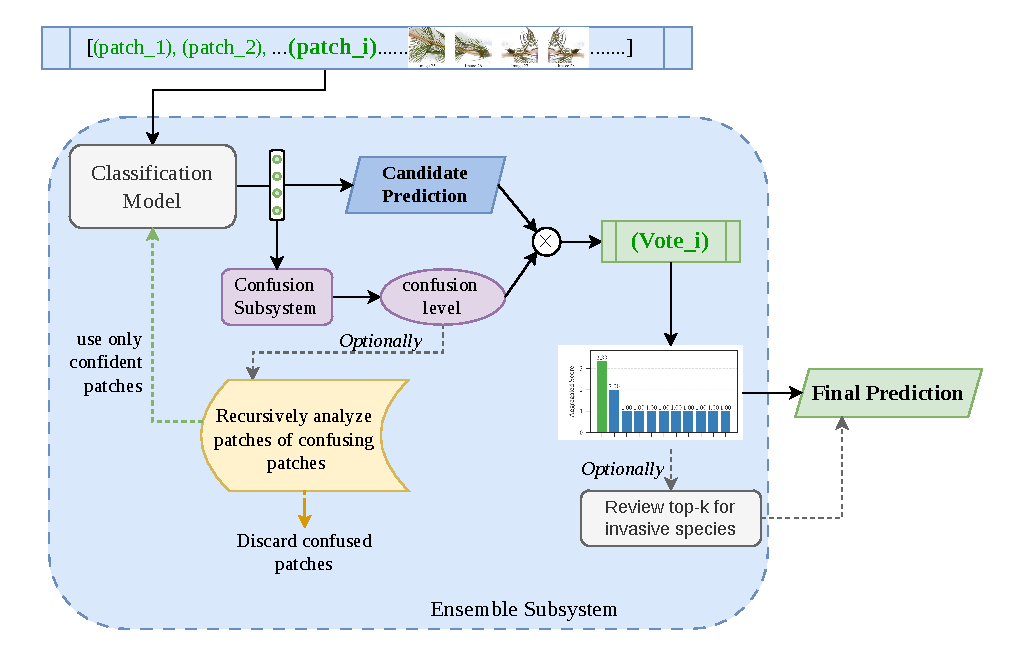
\includegraphics[width=1.0\textwidth]{figs/figs26/ensemble26_simplified.drawio.pdf}
  \caption{Workflow of the Ensemble subsystem. An image flagged for high uncertainty is divided into high-resolution patches. Each patch is processed independently by the classification pipeline and contributes a weighted vote to the final aggregated prediction.}
  \label{fig:ensemble}
\end{figure*}


Each patch is classified independently. Random-resized-crop training makes these partial views admissible inputs. Patch \(i\) with confusion count \(c_i\) contributes a normalized vote
\[
w_i = \frac{c_{\max}-c_i}{c_{\max}}, \qquad c_{\max}=3,
\]
to its predicted class. Accumulated class scores are initialized at \(1\) the first time a class appears, then incremented by \(w_i\). The class with the largest score is returned. If two classes share the maximum, an invasive class is preferred. This is a tie-break, not a top-\(k\) override: YNLT does not replace a unique non-invasive winner with an invasive runner-up.

\subsection{Evaluation Metrics}

During training, the primary indicators used to monitor model convergence were validation accuracy and loss. To prevent the network from generating overconfident predictions, which would compromise the YNLT module's ability to accurately detect uncertainty, label smoothing was applied in conjunction with standard cross-entropy. As demonstrated by \citet{Mulleretal2019}, label smoothing not only improves generalization but also significantly aids in model calibration by preventing the network from assigning full probability to the target class, thereby keeping the logits constrained. The smoothed cross-entropy loss is defined as:

\[
\mathcal{L}_{\text{smooth}} = - \sum_{i=1}^{K} q_i \log p_i
\]
where \( p_i \) is the predicted probability corresponding to class \( i \), \( K \) is the total number of classes, and the smoothed target distribution \( q_i \) is calculated as:

\[
 q_i = (1 - \epsilon) \delta_{i,y} + \frac{\epsilon}{K} 
\]
with \(\epsilon=0.05\) in the reported runs.

Overall model performance was evaluated using standard multi-class metrics, including overall accuracy and class-wise recall. However, given the ecological context of the study, predictions were also aggregated into a binary classification: Invasive (positive class) versus Native (negative class). In this binary framework, the most critical evaluation metric is the False Negative Rate (FNR). The ecological consequences of failing to identify an invasive species (a false negative) severely outweigh the operational costs of misclassifying a native plant as invasive (a false positive). Therefore, minimizing the FNR was a primary objective:
\[
\text{FNR} = \frac{\text{FN}}{\text{TP} + \text{FN}}
\]
where FN represents False Negatives and TP represents True Positives.

To specifically isolate and evaluate the utility of the proposed YNLT block, model predictions were tracked before and after the ensemble process. For any image flagged for high-resolution re-evaluation due to high uncertainty, there are four possible transition outcomes, as outlined in Table \ref{tab:ynlt_outcomes}.

\begin{table}[h]
    \centering
    \begin{tabular}{lcc}
        \hline
        \textbf{Case} & \textbf{Before YNLT} & \textbf{After YNLT} \\
        \hline
        1 & Correct & Correct \\
        2 & Correct & Incorrect \\
        3 & Incorrect & Correct \\
        4 & Incorrect & Incorrect \\
        \hline
    \end{tabular}
    \caption{Possible transition outcomes for images processed by the YNLT ensemble module.}
    \label{tab:ynlt_outcomes}
\end{table}

Based on these transition cases, two custom metrics—Success Rate and Effectiveness—were defined to quantify the module's performance:

\[
\text{Success Rate} = \frac{\text{Total Correct After YNLT}}{\text{Total Images Reviewed by YNLT}}
\]

\[
\text{Effectiveness} = \frac{\text{Transitions from Incorrect to Correct}}{\text{Total Images Reviewed by YNLT}}
\]

These metrics served as key optimization targets for tuning the uncertainty thresholds, as well as the scale and overlap parameters within the patching subsystem.

\subsection{Experimentation}
This section discusses the hyperparameters tuned and some of the design choices that were made in this work 
\subsubsection{Training Classification model}
% learning rate schedule
% AdamW optimizer
% label smoothing
The model was implemented in PyTorch. The original experiment (Table~\ref{tab:ablation}) was trained on a laptop with an NVIDIA RTX A500 GPU (4~GB VRAM) at batch size 4; the experiments of Sections~\ref{subsec:datagrid}--\ref{subsec:curve} were trained on an NVIDIA RTX 3070 Ti (8~GB) at batch size 32 with mixed precision. Only the classification head was trained; all backbone weights remained frozen (27.9~M frozen parameters, 0.26~M trainable for the gated head). Table~\ref{tab:cost} lists the measured cost of each candidate backbone with the gated head, obtained on the RTX 3070 Ti with batch size 1 after warm-up. A single \(224\times 224\) forward pass of ConvNeXt-V2 Tiny requires 4.47~G multiply--adds and 5.2~ms.

This cost is acceptable on a workstation GPU and is the reason the Tiny model was chosen over ViT-B/16, which needs 3.8 times the multiply--adds for the same feature dimension. It is not, by itself, a measurement on the rover's embedded computer. When review is triggered, every retained patch is a separate forward pass: a reviewed image costs about 111 patches, or roughly 200~ms on the RTX 3070 Ti, and the average cost per image therefore depends on how often the uncertainty test fires; the trigger rate is logged for every evaluation. The Nano, Pico and Atto rows of Table~\ref{tab:cost} give the cost of shrinking the backbone, and Section~\ref{subsec:backbones} gives the accuracy, so that the final choice can be made against a measured embedded latency budget.

\begin{table}[h]
    \centering
    \caption{Cost of the candidate frozen backbones with the gated attention head: parameters, multiply--adds for one $224\times 224$ pass, and batch-1 latency on an NVIDIA RTX 3070 Ti. The last column is the latency of one image that YNLT reviews (first pass plus 111 patches in batches of 16); images that are not flagged cost one pass.}
    \label{tab:cost}
    \renewcommand{\arraystretch}{1.2}
    \small
    \begin{tabular}{lrrrrr}
        \hline
        \textbf{Backbone} & \textbf{Params} & \textbf{Trainable} & \textbf{GMACs} & \textbf{ms/pass} & \textbf{ms/review} \\
        \hline
        ConvNeXt-V2 Tiny & 28.1~M & 261{,}933 & 4.47 & 5.2 & 209 \\
        ConvNeXt-V2 Nano & 15.2~M & 218{,}925 & 2.46 & 4.2 & 129 \\
        ConvNeXt-V2 Pico & 8.7~M & 175{,}917 & 1.37 & 3.9 & 94 \\
        ConvNeXt-V2 Atto & 3.5~M & 111{,}405 & 0.55 & 3.9 & 61 \\
        ConvNeXt-V1 Tiny & 28.1~M & 261{,}933 & 4.47 & 3.8 & 153 \\
        ResNet-50 & 24.2~M & 692{,}013 & 4.11 & 3.6 & 129 \\
        EfficientNetV2-B0 & 6.3~M & 433{,}965 & 0.73 & 5.7 & 59 \\
        ViT-B/16 & 86.1~M & 261{,}933 & 16.87 & 5.0 & 383 \\
        \hline
    \end{tabular}
\end{table}

Training used AdamW, cosine learning-rate decay to \(2\times 10^{-5}\), 250 epochs, weight decay \(2\times 10^{-5}\), initial learning rate \(5\times 10^{-4}\), and label smoothing \(\epsilon=0.05\). In the original experiment, model selection used the out-of-distribution validation split. In the new protocol the checkpoint with the highest accuracy on the validation split of the training collection is kept, and the outdoor photographs are never seen before testing. Each configuration is trained with five seeds (8--12); a seed changes the observation-level split and the initialisation of the head.

\subsubsection{Tuning YNLT Block}
YNLT trades accuracy against compute. The scales \(\{0.2,0.3,0.4,0.5\}\) and overlaps \(\{0.0,0.1,0.2,0.3\}\) were held fixed for the reported results. Recursion to still finer patches is implemented but disabled in the experiments here.


%%%%%%%%%%%%%%%%%%%%%%%%%%%%%%%%%%%%%%%%%%%%%%%%%%%%%%%%%%%%
% \begin{table*}[!ht]
% \caption{Summary of YOLO variants with open-source software packages.}
% \label{tab:models}
% \renewcommand{\arraystretch}{1.4}
% \centering
% \resizebox{0.7\textwidth}{!}{
% \begin{tabular}{llll}
% \hline
% Index & YOLO models  & URL & Reference \\ \hline
% 1     & YOLOv3    & \url{https://github.com/ultralytics/YOLOv3}  & \cite{redmon2018YOLOv3}         \\ 
% 2     & YOLOv4    & \url{https://github.com/WongKinYiu/PyTorch-YOLOv4}  & \cite{bochkovskiy2020YOLOv4} \\ 
% 3    & YOLOv5   & \url{https://github.com/ultralytics/YOLOv5}   & \cite{jocher2020YOLOv5}           \\
% 4   & Scaled-YOLOv4     & \url{https://github.com/WongKinYiu/ScaledYOLOv4}   & \cite{wang2021scaled}           \\ 
% 5    & YOLOR      & \url{https://github.com/WongKinYiu/yolor} & \cite{wang2021r}           \\ \hline
% \end{tabular}
% }
% \end{table*}





%%%%%%%%%%%%%%%%%%%%%%%%%%%%%%%%%%%%%%%%%%%%%%%%%%%%%%%%%%%%

\section{Results}
\label{sec:results}


\begin{table*}[!ht]
    \caption{Ablation of the classification head and of YNLT on a shared frozen ConvNeXt-V2 Tiny backbone. Rows differ only in the head (linear vs.\ gated attention) and in whether YNLT is applied at test time. The two YNLT rows use the downsampled patch source of Section~\ref{subsec:patching}. Results are from one stratified 60/20/20 laboratory split (46 test images) and a 17-image OOD test split.}
    \label{tab:ablation}
    \renewcommand{\arraystretch}{1.4}
    \centering
    \resizebox{1.0\textwidth}{!}{
         \begin{tabular}{lcccccc}
             \hline
             \multirow{2}{*}{\textbf{Model}} & \multicolumn{3}{c}{\textbf{Lab Data (\%)}} & \multicolumn{3}{c}{\textbf{OOD Data (\%)}} \\
             \cline{2-4} \cline{5-7}
             & \textbf{Class Acc} & \textbf{Bin Acc} & \textbf{Bin FNR} & \textbf{Class Acc} & \textbf{Bin Acc} & \textbf{Bin FNR} \\
             \hline
             Linear Classifier & 84.78 & 93.48 & 30.0 & 47.06 & 58.82 & 62.5 \\
             Linear + YNLT Block & 91.30 & 93.48 & 30.0 & 52.94 & 58.82 & 62.5 \\
             Gated Attention Classifier & 86.96 & 97.83 & 10.0 & 52.94 & 76.47 & 12.5 \\
             Gated Attention + YNLT Block & 93.48 & 97.83 & 10.0 & 64.71 & 76.47 & 12.5 \\
             \hline
        \end{tabular}
    }
\end{table*}

\subsection{Ablation Tests}
Table~\ref{tab:ablation} isolates the two trainable or test-time components on a shared frozen ConvNeXt-V2 Tiny backbone. The first row is a linear classifier. Adding YNLT to that linear head raises laboratory accuracy from 84.78\% to 91.30\% and OOD accuracy from 47.06\% to 52.94\%, while binary FNR is unchanged. Replacing the linear head with gated attention, still without YNLT, yields a smaller laboratory gain (86.96\%) but a larger OOD gain (52.94\%) and cuts binary FNR from 30.0\% to 10.0\% on the laboratory set and from 62.5\% to 12.5\% on OOD. Combining gated attention with YNLT produces the best 21-way accuracies (93.48\% laboratory, 64.71\% OOD). The two modules are complementary: gated attention mainly reduces invasive false negatives and improves field transfer; YNLT mainly repairs ambiguous 21-way decisions by using high-resolution patches.

All four rows of Table~\ref{tab:ablation} use one stratified split of the 230-image laboratory set and the 33-image field set. A single additional correct prediction on the 46-image laboratory test changes accuracy by about 2.2\%, and on the 17-image field test by 5.9\%; the 95\% confidence half-width of an accuracy near 80\% is about 12 points for 46 images and 19 points for 17. The remaining experiments therefore use five seeds, a 210-image web test split, and the full 42-image outdoor set.

\subsection{Training data and classification head}
\label{subsec:datagrid}

Table~\ref{tab:datagrid} answers the question that motivated the web collection: which combination of training data and head gives the best classifier, and does the answer change with the test domain. Every row uses the frozen ConvNeXt-V2 Tiny backbone and the recipe of Section~\ref{sec:materials_methods}; rows differ in the training collection (laboratory, web, or both), the head (linear, MLP, gated attention), and whether YNLT is applied at test time. Each model is scored on three held-out sets: the laboratory test images (39, identical across rows), the web test images (about 210, grouped by observation), and the 42 outdoor photographs, which no model has seen. Entries are mean \(\pm\) standard deviation over seeds 8--12. Binary accuracy is omitted for space; the released aggregation script prints it.

\begin{table*}[!ht]
    \caption{Training data \(\times\) head \(\times\) YNLT on the frozen ConvNeXt-V2 Tiny backbone. Class accuracy and invasive false negative rate (\%) on the laboratory test (39 images), the web test (about 210 images) and the 42 held-out outdoor photographs; mean \(\pm\) standard deviation over five seeds. YNLT uses the downsampled patch source.}
    \label{tab:datagrid}
    \renewcommand{\arraystretch}{1.3}
    \centering
    \resizebox{1.0\textwidth}{!}{
         \begin{tabular}{llcccccc}
             \hline
             \multirow{2}{*}{\textbf{Training data}} & \multirow{2}{*}{\textbf{Head}} & \multicolumn{2}{c}{\textbf{Lab test}} & \multicolumn{2}{c}{\textbf{Web test}} & \multicolumn{2}{c}{\textbf{Outdoor test}} \\
             \cline{3-4} \cline{5-6} \cline{7-8}
             & & \textbf{Acc} & \textbf{FNR} & \textbf{Acc} & \textbf{FNR} & \textbf{Acc} & \textbf{FNR} \\
             \hline
             % paste the "Training data x head" body printed by scripts/aggregate_results.py --latex
             Lab & Linear & 80.0 $\pm$ 9.0 & 11.1 $\pm$ 7.9 & 17.5 $\pm$ 1.1 & 68.7 $\pm$ 5.1 & 25.7 $\pm$ 4.6 & 86.7 $\pm$ 7.5 \\
             Lab & Linear + YNLT & 80.5 $\pm$ 7.8 & 4.4 $\pm$ 6.1 & 15.5 $\pm$ 1.4 & 63.8 $\pm$ 4.8 & 17.6 $\pm$ 6.2 & 86.7 $\pm$ 7.5 \\
             Lab & MLP & 77.4 $\pm$ 9.5 & 11.1 $\pm$ 11.1 & 18.7 $\pm$ 1.6 & 71.5 $\pm$ 7.9 & 18.6 $\pm$ 8.1 & 90.0 $\pm$ 9.1 \\
             Lab & MLP + YNLT & 76.9 $\pm$ 7.7 & 8.9 $\pm$ 9.3 & 17.1 $\pm$ 2.2 & 65.3 $\pm$ 11.0 & 15.2 $\pm$ 7.1 & 86.7 $\pm$ 13.9 \\
             Lab & Gated attention & 80.5 $\pm$ 11.1 & 13.3 $\pm$ 9.3 & 18.8 $\pm$ 1.7 & 71.2 $\pm$ 5.4 & 25.2 $\pm$ 3.2 & 96.7 $\pm$ 7.5 \\
             Lab & Gated attention + YNLT & 82.6 $\pm$ 8.2 & 2.2 $\pm$ 5.0 & 17.0 $\pm$ 1.7 & 67.1 $\pm$ 4.7 & 15.2 $\pm$ 6.0 & 96.7 $\pm$ 7.5 \\
             \hline
             Web & Linear & 40.0 $\pm$ 4.7 & 37.8 $\pm$ 9.9 & 54.3 $\pm$ 4.9 & 36.5 $\pm$ 7.1 & 36.2 $\pm$ 7.0 & 53.3 $\pm$ 21.7 \\
             Web & Linear + YNLT & 37.9 $\pm$ 4.2 & 28.9 $\pm$ 6.1 & 51.5 $\pm$ 5.2 & 28.2 $\pm$ 10.2 & 31.9 $\pm$ 6.0 & 46.7 $\pm$ 21.7 \\
             Web & MLP & 36.9 $\pm$ 5.9 & 44.4 $\pm$ 11.1 & 55.9 $\pm$ 5.6 & 36.5 $\pm$ 13.8 & 31.4 $\pm$ 3.1 & 66.7 $\pm$ 16.7 \\
             Web & MLP + YNLT & 36.9 $\pm$ 4.3 & 26.7 $\pm$ 12.7 & 54.1 $\pm$ 5.9 & 25.4 $\pm$ 10.3 & 32.4 $\pm$ 4.9 & 43.3 $\pm$ 19.0 \\
             Web & Gated attention & 38.5 $\pm$ 4.8 & 40.0 $\pm$ 12.7 & 55.5 $\pm$ 5.2 & 37.7 $\pm$ 5.6 & 32.9 $\pm$ 9.3 & 63.3 $\pm$ 18.3 \\
             Web & Gated attention + YNLT & 37.4 $\pm$ 3.4 & 24.4 $\pm$ 14.5 & 54.4 $\pm$ 4.5 & 24.1 $\pm$ 8.3 & 31.9 $\pm$ 4.6 & 36.7 $\pm$ 13.9 \\
             \hline
             Lab + web & Linear & 81.5 $\pm$ 8.0 & 13.3 $\pm$ 12.2 & 57.7 $\pm$ 4.4 & 33.2 $\pm$ 6.3 & 35.2 $\pm$ 2.6 & 63.3 $\pm$ 13.9 \\
             Lab + web & Linear + YNLT & 75.4 $\pm$ 9.2 & 2.2 $\pm$ 5.0 & 54.6 $\pm$ 5.2 & 22.9 $\pm$ 7.3 & 35.7 $\pm$ 3.4 & 36.7 $\pm$ 7.5 \\
             Lab + web & MLP & 75.4 $\pm$ 6.9 & 11.1 $\pm$ 7.9 & 56.1 $\pm$ 5.5 & 37.0 $\pm$ 10.7 & 33.3 $\pm$ 4.5 & 60.0 $\pm$ 19.0 \\
             Lab + web & MLP + YNLT & 75.4 $\pm$ 6.9 & 2.2 $\pm$ 5.0 & 54.0 $\pm$ 5.2 & 28.4 $\pm$ 7.4 & 32.9 $\pm$ 3.1 & 40.0 $\pm$ 9.1 \\
             Lab + web & Gated attention & 83.6 $\pm$ 5.0 & 6.7 $\pm$ 9.9 & 56.3 $\pm$ 4.6 & 35.7 $\pm$ 8.5 & 31.4 $\pm$ 5.2 & 70.0 $\pm$ 13.9 \\
             Lab + web & Gated attention + YNLT & 81.0 $\pm$ 6.7 & 2.2 $\pm$ 5.0 & 55.5 $\pm$ 4.3 & 26.2 $\pm$ 6.1 & 32.4 $\pm$ 5.5 & 36.7 $\pm$ 18.3 \\
             \hline
        \end{tabular}
    }
\end{table*}

Three comparisons are of interest. First, the training collection decides the test domain. Models trained on laboratory images alone reach 77--83\% on the laboratory test but 17--19\% on the web test and 19--26\% on the outdoor photographs: the white-background features do not transfer. Training on the web images alone reverses the picture (54--56\% web, 31--36\% outdoor, but only 37--40\% laboratory). Training on both keeps laboratory accuracy (81.5\% linear, 83.6\% gated, against 80.0\% and 80.5\% with laboratory data only), triples web accuracy to 56--58\% and lifts outdoor accuracy to 31--36\%. Adding field photographs therefore costs nothing on the laboratory test and is the single largest effect in the table. Second, at matched data the head matters little. On lab+web the linear, MLP and gated heads are within one standard deviation of one another on every accuracy column; the gated head has the best laboratory accuracy (83.6 \(\pm\) 5.0\%) and the lowest laboratory invasive FNR without YNLT (6.7\% against 13.3\% for the linear head), while the linear head is one to four points higher on the web and outdoor tests, differences the seed spread does not resolve. Sixteen times more weights neither help nor hurt at 834 training images, and the ablation of Table~\ref{tab:ablation}, where the gated head improved field accuracy on one split, does not survive five seeds. Third, YNLT trades 21-way accuracy for invasive recall. On lab+web it lowers laboratory accuracy by 2.6 points (gated) to 6.1 points (linear) and web accuracy by one to three points, and leaves outdoor accuracy unchanged, but it cuts the invasive FNR on every test set: laboratory 13.3\(\to\)2.2\% (linear) and 6.7\(\to\)2.2\% (gated), web 33\(\to\)23\% and 36\(\to\)26\%, outdoor 63\(\to\)37\% and 70\(\to\)37\%. The review is triggered for 14--21\% of laboratory, 31--34\% of web and 38--41\% of outdoor images, and the mean cost including unreviewed images is 91--148~ms per laboratory image, 104--189~ms per web image and 120--242~ms per outdoor image on the RTX 3070 Ti, against 5~ms for a single pass. The outdoor column should be read with its size in mind: 42 images, 16 of a single species, and six invasive examples, so its FNR moves in steps of about 17 points and its accuracy in steps of 2.4.

\subsection{Backbone comparison}
\label{subsec:backbones}

Table~\ref{tab:backbones} replaces the frozen encoder and keeps the linear head, the training recipe, and the lab+web training collection, with three seeds per encoder. The encoders are the ConvNeXt-V2 family (Tiny, Nano, Pico, Atto), ConvNeXt-V1 Tiny (\texttt{convnext\_tiny.fb\_in22k\_ft\_in1k}), ResNet-50 (\texttt{resnet50.a1\_in1k}), EfficientNetV2-B0 (\texttt{tf\_efficientnetv2\_b0.in1k}), and ViT-B/16 (\texttt{vit\_base\_patch16\_224.augreg\_in21k\_ft\_in1k}). The smaller ConvNeXt-V2 members are also trained with the gated head, since they are the candidates for the rover if the Tiny model does not meet the onboard budget. Read together with Table~\ref{tab:cost}, this table gives accuracy per unit of compute, which is the quantity that matters for deployment.

\begin{table*}[!ht]
    \caption{Frozen encoders on the lab+web training collection, linear head unless stated, three seeds (8--10). Class accuracy and invasive FNR (\%) on the laboratory, web and outdoor test sets; mean \(\pm\) standard deviation. Costs are in Table~\ref{tab:cost}.}
    \label{tab:backbones}
    \renewcommand{\arraystretch}{1.3}
    \centering
    \resizebox{1.0\textwidth}{!}{
         \begin{tabular}{llcccccc}
             \hline
             \multirow{2}{*}{\textbf{Encoder}} & \multirow{2}{*}{\textbf{Head}} & \multicolumn{2}{c}{\textbf{Lab test}} & \multicolumn{2}{c}{\textbf{Web test}} & \multicolumn{2}{c}{\textbf{Outdoor test}} \\
             \cline{3-4} \cline{5-6} \cline{7-8}
             & & \textbf{Acc} & \textbf{FNR} & \textbf{Acc} & \textbf{FNR} & \textbf{Acc} & \textbf{FNR} \\
             \hline
             % paste the "Other encoders" body printed by scripts/aggregate_results.py --latex;
             % the Tiny rows are the lab+web / seeds 8-10 subset of the data suite (--seeds 8 9 10).
             ConvNeXt-V2 Tiny & Linear & 82.9 $\pm$ 9.7 & 7.4 $\pm$ 12.8 & 56.0 $\pm$ 3.3 & 36.6 $\pm$ 5.0 & 34.9 $\pm$ 2.7 & 66.7 $\pm$ 16.7 \\
             ConvNeXt-V2 Nano & Linear & 75.2 $\pm$ 9.7 & 7.4 $\pm$ 12.8 & 52.9 $\pm$ 3.6 & 46.2 $\pm$ 4.2 & 33.3 $\pm$ 8.6 & 61.1 $\pm$ 19.2 \\
             ConvNeXt-V2 Pico & Linear & 61.5 $\pm$ 6.8 & 40.7 $\pm$ 17.0 & 40.2 $\pm$ 4.0 & 51.0 $\pm$ 5.2 & 22.2 $\pm$ 3.6 & 72.2 $\pm$ 9.6 \\
             ConvNeXt-V2 Atto & Linear & 56.4 $\pm$ 18.5 & 59.3 $\pm$ 17.0 & 38.5 $\pm$ 1.9 & 48.8 $\pm$ 13.4 & 27.8 $\pm$ 5.5 & 16.7 $\pm$ 0.0 \\
             ConvNeXt-V1 Tiny & Linear & 78.6 $\pm$ 5.3 & 7.4 $\pm$ 6.4 & 53.6 $\pm$ 6.3 & 41.3 $\pm$ 7.8 & 47.6 $\pm$ 4.1 & 55.6 $\pm$ 25.5 \\
             ResNet-50 & Linear & 59.0 $\pm$ 6.8 & 29.6 $\pm$ 17.0 & 40.4 $\pm$ 5.1 & 42.8 $\pm$ 6.4 & 22.2 $\pm$ 5.0 & 33.3 $\pm$ 16.7 \\
             EfficientNetV2-B0 & Linear & 60.7 $\pm$ 3.9 & 37.0 $\pm$ 6.4 & 36.2 $\pm$ 4.6 & 49.6 $\pm$ 9.4 & 14.3 $\pm$ 2.4 & 61.1 $\pm$ 25.5 \\
             ViT-B/16 & Linear & 74.4 $\pm$ 5.1 & 22.2 $\pm$ 11.1 & 51.5 $\pm$ 3.5 & 44.9 $\pm$ 9.4 & 32.5 $\pm$ 7.3 & 44.4 $\pm$ 19.2 \\
             \hline
             ConvNeXt-V2 Tiny & Gated attention + YNLT & 80.3 $\pm$ 7.8 & 0.0 $\pm$ 0.0 & 56.9 $\pm$ 2.3 & 28.4 $\pm$ 7.3 & 29.4 $\pm$ 3.6 & 38.9 $\pm$ 19.2 \\
             ConvNeXt-V2 Nano & Gated attention + YNLT & 75.2 $\pm$ 7.8 & 0.0 $\pm$ 0.0 & 50.1 $\pm$ 2.7 & 31.9 $\pm$ 6.0 & 26.2 $\pm$ 2.4 & 38.9 $\pm$ 9.6 \\
             ConvNeXt-V2 Pico & Gated attention + YNLT & 70.9 $\pm$ 5.3 & 22.2 $\pm$ 11.1 & 39.9 $\pm$ 1.0 & 37.4 $\pm$ 10.4 & 21.4 $\pm$ 10.4 & 66.7 $\pm$ 28.9 \\
             ConvNeXt-V2 Atto & Gated attention + YNLT & 60.7 $\pm$ 14.6 & 25.9 $\pm$ 12.8 & 39.9 $\pm$ 1.7 & 39.4 $\pm$ 5.4 & 28.6 $\pm$ 4.8 & 33.3 $\pm$ 16.7 \\
             \hline
        \end{tabular}
    }
\end{table*}

ConvNeXt-V2 Tiny is the most accurate encoder on the laboratory (82.9\%) and web (56.0\%) tests and, read against Table~\ref{tab:cost}, the best accuracy per unit of compute among the models that reach 50\% on the web test. ViT-B/16 costs 3.8 times the multiply--adds and is lower on every column (74.4\%, 51.5\%, 32.5\%). ResNet-50 and EfficientNetV2-B0, pretrained on ImageNet-1k only, lose 20 points or more on every test set, which points to the ImageNet-22k pretraining rather than the convolutional design as the source of the advantage; ConvNeXt-V1 Tiny, which shares that pretraining, is within four points of V2 on the laboratory and web tests and is the best encoder on the outdoor photographs (47.6 \(\pm\) 4.1\% against 34.9\%), a difference of about five of the 42 images that merits a larger outdoor collection before it is interpreted. Within the ConvNeXt-V2 family the cost of shrinking is steep below Nano. Nano keeps 91\% of Tiny's laboratory accuracy and 94\% of its web accuracy for 55\% of the multiply--adds and 62\% of the review latency (129 against 209~ms); Pico and Atto fall to 56--62\% laboratory and 38--40\% web accuracy, so their 3--8 times lower cost buys a different classifier rather than a cheaper version of the same one. With the gated head and YNLT, Nano reaches a laboratory invasive FNR of 0\% on all three seeds at 75\% laboratory accuracy, which makes it the fallback for the rover if the Tiny model does not meet the onboard budget.

\subsection{Learning curve}
\label{subsec:curve}

Figure~\ref{fig:curve} addresses the sample-size question of Section~\ref{subsec:capacity} directly. The linear and gated heads were trained on 10\%, 25\%, 50\% and 100\% of the lab+web training split, whole observations at a time and at least one observation per species, with the validation and test splits held fixed, for three seeds each. Where a curve flattens, additional images of the kind we can collect stop paying off; where the gated curve lies above the linear one at small fractions, the extra 246~k weights are not costing data efficiency.

\begin{figure*}[!ht]
  \centering
  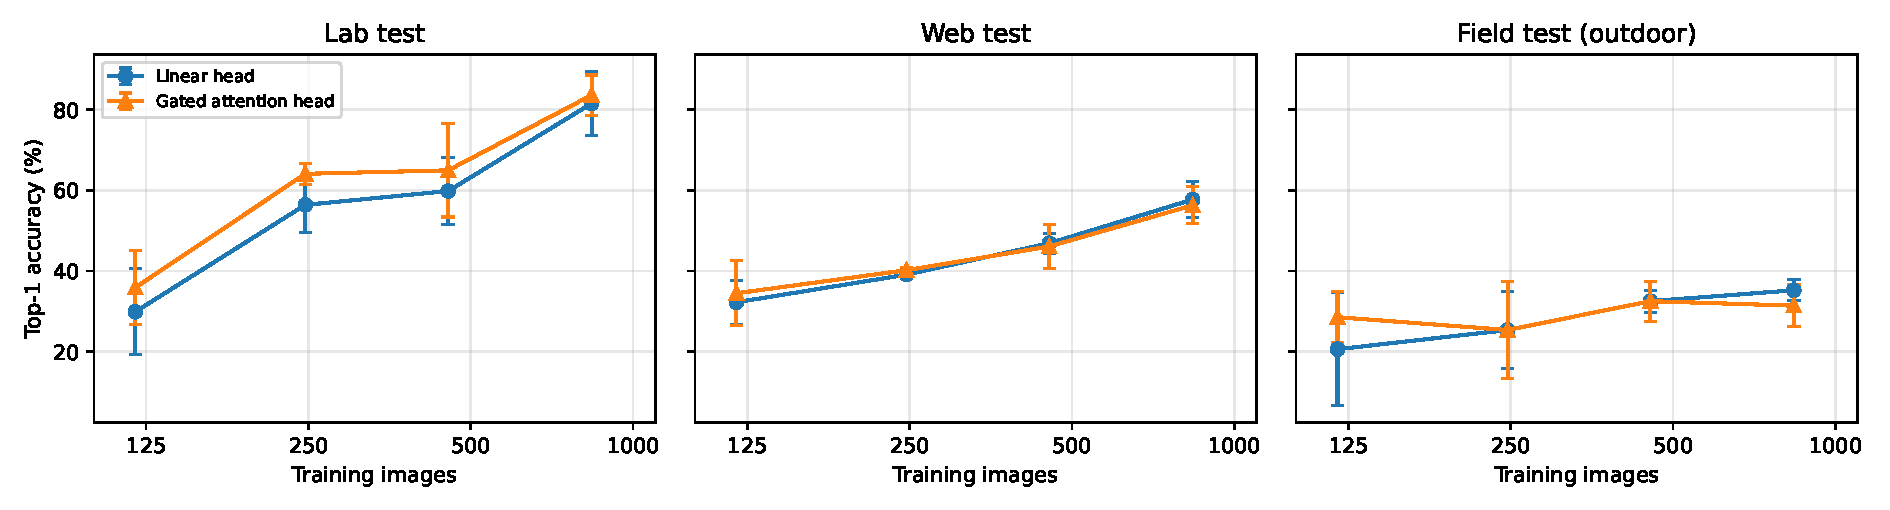
\includegraphics[width=1.0\textwidth]{figs/learning_curve.pdf}
  \caption{Test accuracy against the number of training images for the linear and gated attention heads on the frozen ConvNeXt-V2 Tiny backbone (lab+web collection; mean \(\pm\) standard deviation over three seeds; first pass only). Panels: laboratory test, web test, outdoor test.}
  \label{fig:curve}
\end{figure*}

The four points correspond to about 6, 12, 22 and 40 training images per class. Neither the laboratory nor the web curve has flattened: laboratory accuracy rises from 30\% (linear) and 36\% (gated) at 6 images per class to 82\% and 84\% at 40, and web accuracy from 32--35\% to 56--58\%, gaining roughly ten points per doubling of the training set with no sign of saturation at the full collection. The outdoor curve behaves differently: it rises from 21--29\% to 33\% by 22 images per class and then stays at 31--35\%, so for the unseen hand-held photographs the limit is the domain of the training images, not their number. The gated head is not more data-hungry than the linear one despite its sixteen-fold weight count; it is six to eight points higher at 6 and 12 images per class on the laboratory test and level with the linear head elsewhere, consistent with the capacity argument of Section~\ref{subsec:capacity}: on a frozen 768-dimensional representation the number of images per class, not the number of head weights, governs the fit. For the laboratory and web domains the practical answer to the sample-size question is therefore ``more than we have'': a further doubling to about 80 images per class is expected to add several points, whereas the outdoor domain needs a different kind of image rather than more of the same.

\subsection{Best Model Performance}

The last row in Table \ref{tab:ablation} shows that the best performing model is a combination of a Gated Attention based classification head on a ConvNeXt-V2 backbone for feature extraction, along with the proposed YNLT block. In this section we will look at the performance of this model in detail.

% Example - Figure 1 - Image and classification scores
\begin{figure*}[!h]
  \centering
  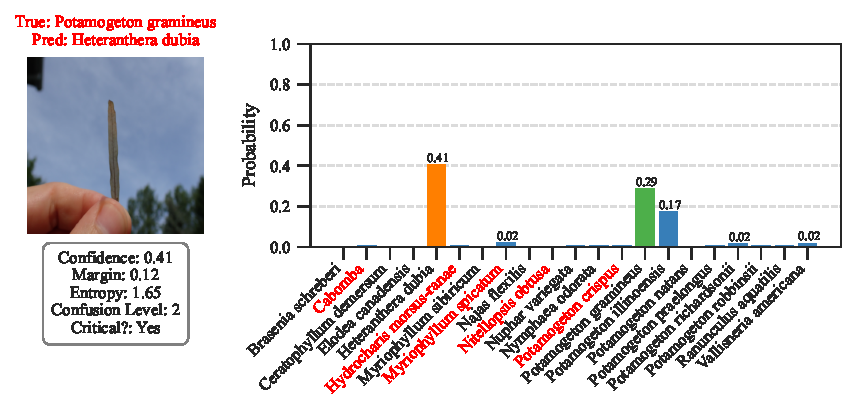
\includegraphics[width=1.0\textwidth]{figs/sample_prediction_initial.pdf}
  \caption{Example of an initially misclassified image. The bar chart shows the model’s output probabilities, where the highest logit corresponds to Heteranthera dubia while the true label is Potamogeton gramineus. The uncertainty metrics (bottom left) indicate model confusion and trigger the YNLT block to re-examine the image. The corrected prediction after the second pass is shown in the following figure.}
  \label{fig:incorrect}
\end{figure*}
%The figure shows a detailed report of one of the images that was initially classified incorrectly. The bar graph on the right shows the probability distribution from the output of the classification model. The highest logit corresponds to Heteranthera dubia, but the image actually is of Potamogeton gramineus. Even though the model is wrong, it accurately communicates that it is confused through the metrics listed in the box at the bottom left. This signals the YNLT block to take a second closer look at the image. In this particular example, the revised prediction after a second look was correct, as seen in the next figure.


The first component of our solution is the classification model that taken an input image and outputs logits corresponding to the probabilities of the image belonging to each of the 21 species of plants. Figure \ref{fig:incorrect} illustrates this stage with a sample image belonging to the Potamogeton gramineus species from the out-of-distribution test set. The bar graph in \ref{fig:incorrect} represents the probability distribution from the output of the classification model. We observe that the second highest predicted probability actually corresponds to the correct species. Even though this initial prediction is wrong, the model is not very confident with this prediction. The confidence is only 0.41, and the margin, which is the difference between the confidence score and that of the second highest prediction is 0.12. In this particular example, the entropy of the distribution which is also one of the metrics used to evaluate confusion is not very high. It is at moderate value of 1.65. But because two of the three metrics signal that the model is confused, the image is passed on to the YNLT block before a final prediction is made.

% Example - Image 2 - YNLT Aggregate Voting scores
\begin{figure}[!h]
  \centering
  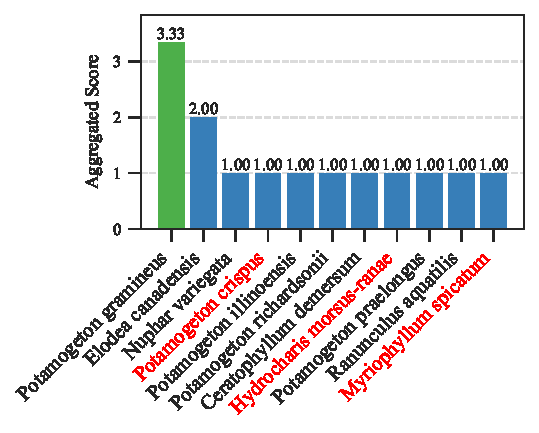
\includegraphics[width=0.48\textwidth]{figs/sample_prediction_final.pdf}
  \caption{The figure shows the aggregated scores from the voting in the Ensemble subsystem that was done for the image in the previous figure. Potamogeton gramineus is the revised final prediction with the highest votes, which in this particular example is correct.}
  \label{fig:ynlt_corrected}
\end{figure}

The second component of our solution as illustrated in \ref{fig:ensemble} first creates patches from the original high-resolution version of the current image, and then aggregates votes weighted by the confidence level of each patch. For the sample image discussed in Figure \ref{fig:incorrect}, the aggregate scores from this step are shown in Figure \ref{fig:ynlt_corrected}. The highest score corresponds to the Potamogeton gramineus species, which turns out to be the correct prediction for this image.

% Confusion matrices and classwise analysis

% \begin{figure}[!h]
%   \centering
%   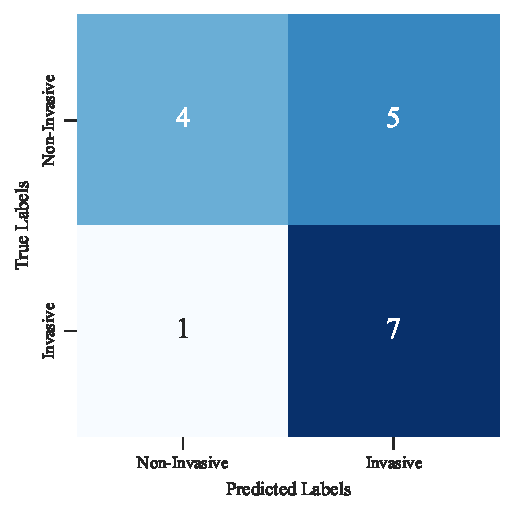
\includegraphics[width=0.45\textwidth]{figs/figs26/ood_binary_cm.pdf}
%   \caption{Binary Confusion Matrix on the out-of-distribution test set of crowd-sourced images. Binary categories were created by grouping all the native and invasive plant species together.}
%   \label{fig:bin_cm}
% \end{figure}

% \begin{figure*}[!h]
%   \centering
%   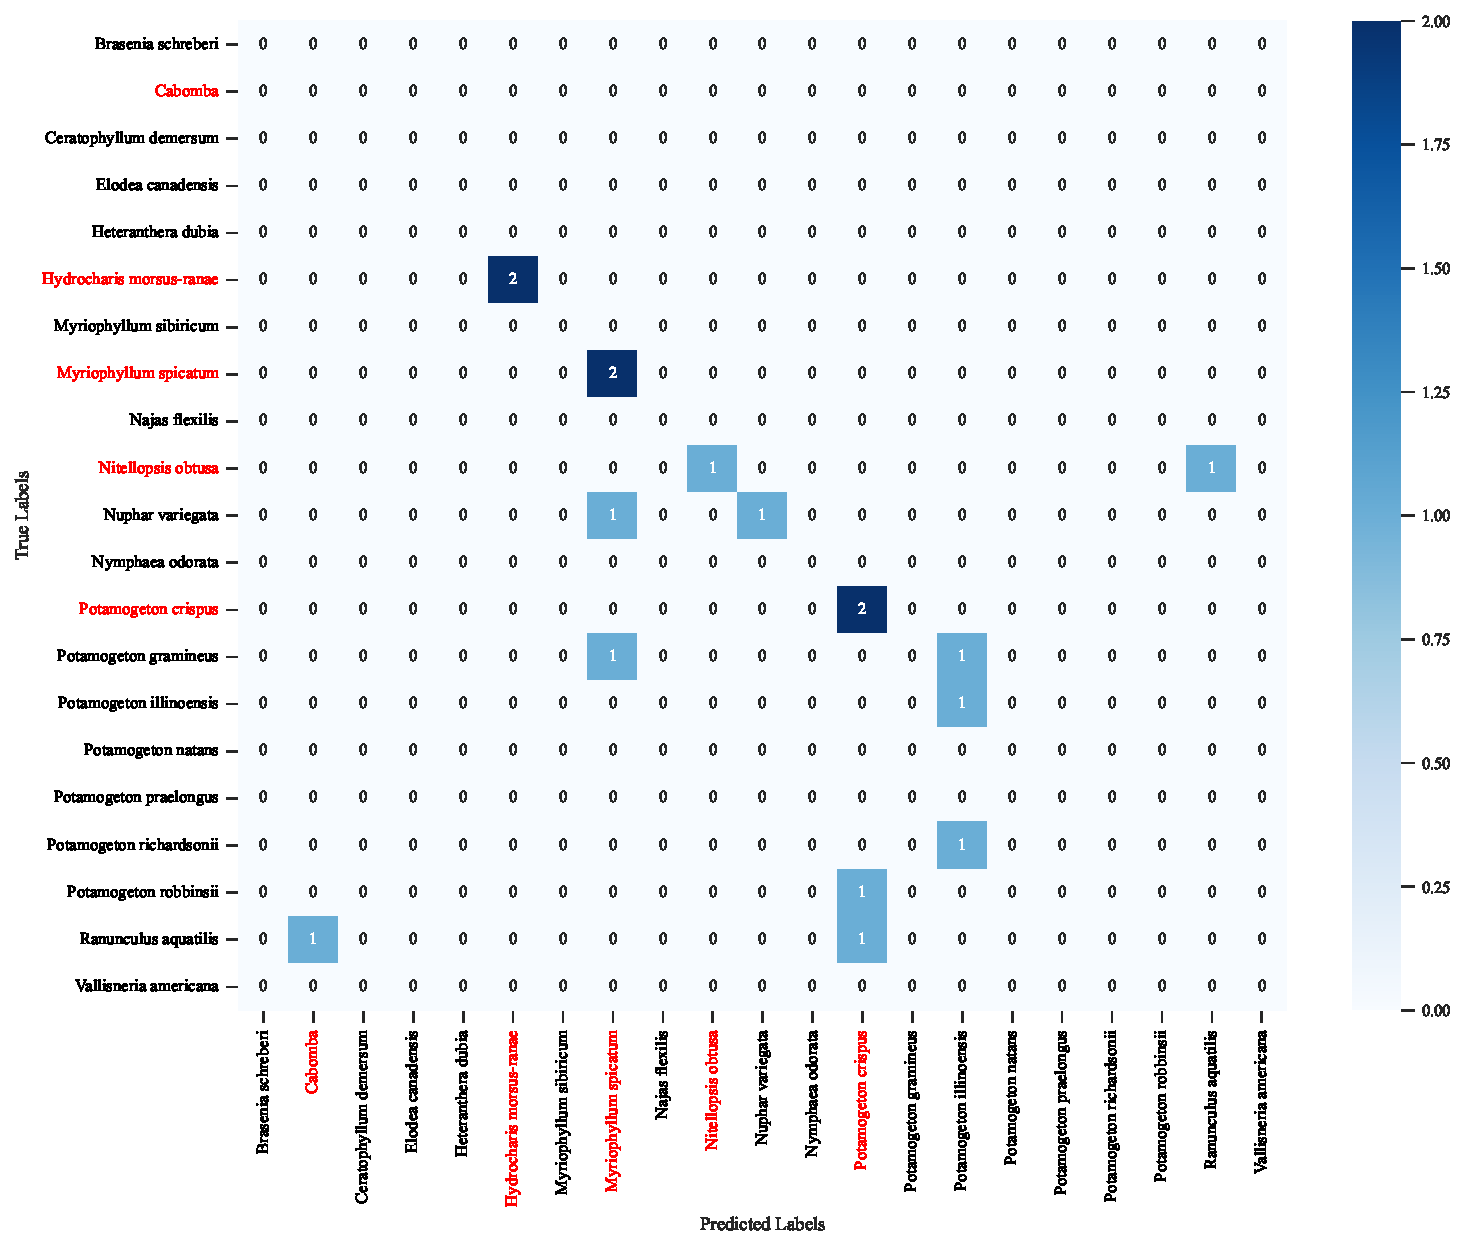
\includegraphics[width=1.0\textwidth]{figs/figs26/ood_classwise_cm.pdf}
%   \caption{The figure tabulates the classwise confusion matrix of the predictions made on the out-of-distribution test set. The numbers on the diagonal represent correct predictions. We can also see which species the model gets confused between from the non-diagonal entries.}
%   \label{fig:classwise_butterfly}
% \end{figure*}


% \begin{figure*}[!h]
%   \centering
%   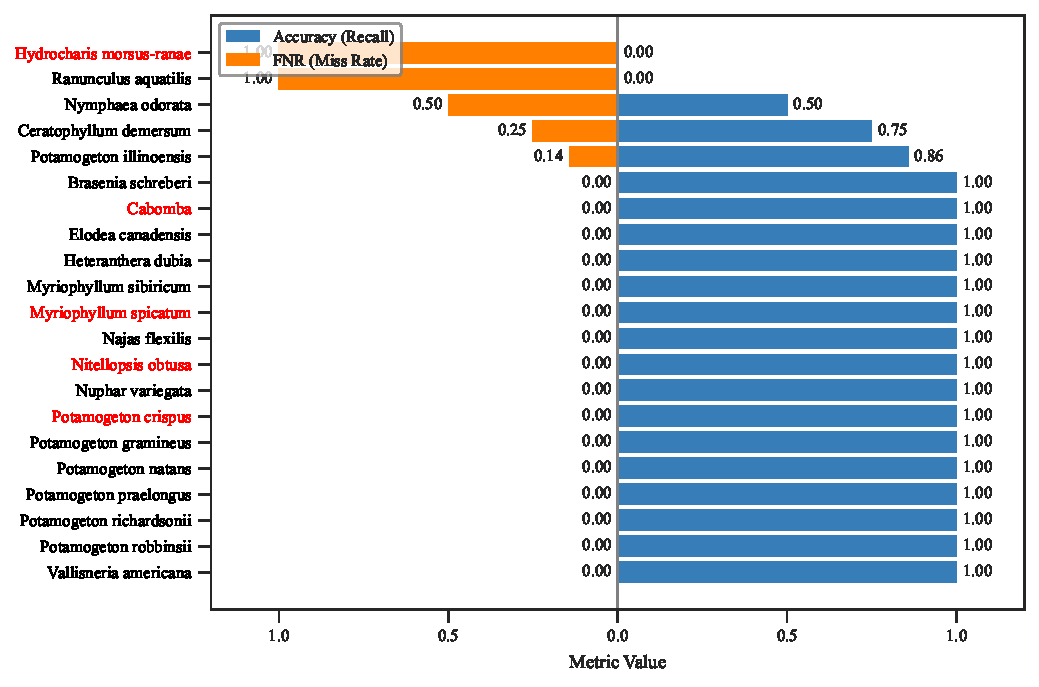
\includegraphics[width=1.0\textwidth]{figs/figs26/lab_butterfly_chart.pdf}
%   \caption{The figure is a butterfly bar graph representing classwise metrics on the best model's performance on the test set.The two metrics here are Recall or accuracy, which we are trying to maximize, and the False Negative Rate, which we aim to minimize. It can be observed that the model performs reasonably well on all classes except Hydrocharis morsus-ranae.}
%   \label{fig:classwise_butterfly}
% \end{figure*}

\section{Discussion}

\textbf{Overcoming Data Scarcity through Scale-Invariant Patching}
The primary challenge in applying deep learning to aquatic plant identification is the high cost of acquiring large, annotated datasets from underwater environments. While laboratory and crowd-sourced images are more accessible, models trained on small datasets of high-resolution images often suffer from the curse of dimensionality when downsampled to standard input sizes. This study addressed this limitation by implementing a probabilistic crop and resize augmentation strategy. By training the model on overlapping patches ranging from 20\% to 100\% of the original image size, the network learned scale-invariant representations of fine morphological details. This approach allowed the model to maximize the utility of the limited 230-image laboratory dataset without losing critical botanical features during standard downsampling.

\textbf{Architectural Suitability for Domain Generalization}
The choice of the ConvNeXt-V2 backbone and the custom Gated Attention head was critical for generalizing from controlled laboratory settings to out-of-distribution crowd-sourced images. ConvNeXt-V2 provided a parameter-efficient foundation, minimizing the risk of overfitting. Furthermore, its pretraining on ImageNet-22k included hierarchical classifications of aquatic plants such as pondweeds and waterlilies. This extensive pretraining equipped the backbone with highly relevant feature extraction capabilities before fine-tuning. However, because these extracted features also contain domain-specific background noise from the laboratory environment, the Gated Attention head was introduced. By explicitly learning to suppress background artifacts and isolate plant-specific signals, the attention mechanism enabled the model to maintain robust performance across varying environments, contributing directly to the 64.71\% accuracy achieved on the unseen crowd-sourced dataset.

\textbf{Addressing Uncertainty with the YNLT Module}
Standard downsampling often obscures the subtle visual distinctions between native and invasive aquatic species. The proposed `You Need To Look Twice' (YNLT) module resolved this by selectively extracting and ensembling high-resolution patches only when the initial prediction exhibited high uncertainty. For this mechanism to function effectively, the model's confidence scores needed strict calibration. The integration of label smoothing during training prevented the network from generating overconfident incorrect predictions, ensuring that visual ambiguity triggered the YNLT re-evaluation rather than being ignored. By dynamically shifting focus to localized, high-resolution features, the YNLT module successfully corrected ambiguous predictions and played a central role in minimizing the False Negative Rate, a critical metric for invasive species management.

\textbf{Training data and model selection}
Optimizing purely for laboratory validation accuracy often degrades field performance. The original experiment therefore selected checkpoints on an out-of-distribution validation split. With the web collection available, field conditions enter training directly and the outdoor photographs can be kept entirely unseen, which is the cleaner test of laboratory-to-field transfer. The web images are not underwater photographs either, so the data-source ablation measures transfer from laboratory and hand-held field imagery to unseen hand-held imagery; underwater footage from the rover remains the target domain that no current collection covers.

\textbf{Weights, samples and what the learning curve says}
The question of how many images the trained weights require has a measured answer rather than a rule. Only 16~k to 262~k head weights are fitted on a frozen 768-dimensional representation; such a probe is governed by images per class, and the learning curve (Figure~\ref{fig:curve}) shows where additional images stop improving each test domain. At 40 training images per class the laboratory and web curves are still rising by about ten points per doubling, so the present collection is below the saturation point for both, while the outdoor curve flattens at about 22 images per class because the remaining error is a domain gap rather than a sample-size gap. The gated head, with sixteen times the weights of the linear head, is no more data-hungry and is slightly better at the smallest fractions, so the number of head weights is not the quantity to budget for; images per class is. The test sets bound what can be concluded: with 39 laboratory and 42 outdoor images a single run cannot resolve differences smaller than about 15 points, which is why five seeds and the 210-image web test are reported.

\textbf{Computational cost and edge deployment}
The target platform is a camera-equipped underwater rover, and it shaped the architecture: a compact frozen convolutional encoder, a head that is cheap to retrain, and a second look that is spent only on uncertain images. A frozen ConvNeXt-V2 Tiny encoder plus the gated head contains 28.1~M parameters, of which 0.26~M are trained. One \(224\times 224\) forward pass is 4.47~G multiply--adds and 5.2~ms on the RTX 3070 Ti used for Table~\ref{tab:cost}; it also runs on the 4~GB laptop GPU used for the original training. YNLT does not change the parameter count, but it multiplies inference cost by the number of patches on the subset of images with \(c\ge 1\): with the multi-scale schedule that is 111 additional forward passes, or about 200~ms, for each reviewed image. The average cost per image is therefore one forward pass plus the trigger rate times that review cost, and the released code logs the trigger rate for every evaluation so this quantity is measured rather than assumed. Table~\ref{tab:cost} and Section~\ref{subsec:backbones} give the cost and the accuracy of the Nano, Pico and Atto members of the same family, so that the backbone can be chosen against the rover's measured latency budget. That budget has not yet been measured on the embedded computer; until it is, workstation and laptop inference is the demonstrated operating regime.

\textbf{Limitations and Future Work}
The primary limitation remains dataset size and domain. Several classes have only two or three laboratory images, which rules out stratified five-fold cross-validation and leaves one laboratory training image for the rarest species. Table~\ref{tab:ablation} is one split of the 230/33 collection and is not reproduced by the retraining runs on the 203/42 folders. The web collection raises the per-class count to 37--123 images, but it is crowd-sourced, dominated by surface and hand-held views, biased toward North America and Europe, and about 80\% of it carries non-commercial or no-derivative licences, so it can be used for research but not redistributed as a dataset. The outdoor test covers 9 of 21 species. Full-resolution patches matched the downsampled vote on accuracy at five to ten times the cost, so they are not used, but a lighter full-resolution schedule may still help on photographs where the plant is small. A biology-specific encoder such as BioCLIP has not been run. Future training may use unlabeled underwater footage from the rover before the supervised head is fit, and embedded latency must be measured before a backbone is fixed.

\textbf{Broader Impacts}
Deployed on a laptop or a field computer, these models can assist screening of photographs before a botanist confirms the record. The same head and backbone are the candidates for onboard screening on an underwater rover once the embedded latency budget is measured, and Table~\ref{tab:cost} provides the smaller backbones to fall back on if the Tiny model does not fit.



%%%%%%%%%%%%%%%%%%%%%%%%%%%%%%%%%%%%%%%%%%%%%%%%%%%%%%%%%%%%%%%%%%%%%%%%%%%%%%%%%%%%%%
\section{Conclusion}
\label{sec:conclu}
% summarise work - data and main contributions
% applications and broader impact 
This study set out to classify 21 Michigan aquatic plant species, five of them invasive, with a model small enough to run on an underwater rover and trained from the few images that such a problem affords. A frozen ConvNeXt-V2 Tiny backbone (28~M parameters, 4.47~G multiply--adds per image), a gated attention head of 0.26~M trained weights, and a confidence-aware second-look module (YNLT) raised laboratory accuracy from 84.78\% to 93.48\% and field accuracy from 47.06\% to 64.71\% on a single stratified split of 230 laboratory and 33 field images. YNLT is not a new backbone. It is a test-time rule that spends extra computation only when the first look is uncertain, which is the setting where small laboratory models fail under domain shift.

To put that result on firmer ground, 1{,}140 openly licensed field photographs of the same species were added from GBIF-mediated iNaturalist observations, split by observation to prevent leakage, and the training collection, the head, the backbone and the number of training images were varied with five seeds and three held-out test sets (Tables~\ref{tab:datagrid}--\ref{tab:backbones}, Figure~\ref{fig:curve}). Training on laboratory and web images together is the best combination: it keeps laboratory accuracy at 82--84\%, triples web accuracy to 56--58\% and raises outdoor accuracy from about 25\% to about 35\%, while the choice of head changes accuracy by less than the seed spread and YNLT cuts the invasive false negative rate on every test set (to 2\% on the laboratory test and from 63--70\% to 37\% outdoors) at a cost of a few points of 21-way accuracy. ConvNeXt-V2 Tiny remains the best encoder per unit of compute; Nano keeps more than 90\% of its accuracy at 55\% of the cost, whereas Pico and Atto lose 20 points or more. The learning curves are still rising at 40 images per class on the laboratory and web tests and flatten only on the outdoor test, so the collection should grow further for the former and change domain for the latter. The trainable weights number 16~k to 262~k; the experiments show how many images per class they need rather than appealing to a rule. Measured inference cost on the rover's embedded computer is the remaining deployment step; until it exists, the method is a laptop-scale screening tool for fisheries and environmental monitoring, with the backbone family and measurements in place to make the onboard choice.



\section*{Authorship Contribution}

\textbf{Aaryan Panigrahi}: Formal analysis, Software, Writing - original draft; \\
\textbf{Fengying Dang}: Conceptualization, Investigation, Data curation, Supervision, Writing - original \& draft \& review \& editing.  

\section*{Acknowledgement}
The authors thank Dr. Jo Latimore for providing the weed images that supported the experimental evaluation.

% This work was supported in part by ???. 
% helping annotate the weed images and Dr. ??? for the assistance in weed identification. 

\typeout{}
% \bibliographystyle{model1-num-names}
\bibliography{ref}
\end{document}

